\documentclass[spanish,letterpaper,12pt,twoside,openany]{article}
\usepackage[spanish, activeacute]{babel}
\usepackage{babelbib}
\usepackage{etoolbox}
\patchcmd\btxselectlanguage{\csname}{\csname TEMPPATCH}{}{} % Para hacer a babelbib funcionar
\usepackage[utf8]{inputenc}
%\usepackage[ansinew]{inputenc}
\usepackage{amstext, amssymb, amsthm, amsmath, amsbsy}%, asmsfonts}
\usepackage{tabularx}
\usepackage[margin=20pt,font=small,labelfont=bf,labelsep=period]{caption}%%Para modificar el formato del texto de los "caption"
\usepackage{graphicx}
\usepackage{url}
\usepackage{listings}%%Para incluir codigo
\usepackage[final]{pdfpages}%%Para incluir archivos en pdf
\usepackage{geometry}
\usepackage [round]{natbib}
\usepackage{enumerate}
\usepackage{subfig}%%Para incluir subgraficos
\usepackage[pdftex, pdftitle={Propuesta Doctorado Juan Carlos Vergara Gallego}, pdfauthor={J. Vergara}, pdfsubject={Propuesta de Doctorado}, pdfkeywords={Efectos Topograficos, Efectos de Sitio, Microzonificaci\'on Sismica, Propagacion de Ondas, Mecanica Computacional, Metodo de Elementos Finitos, Metodo de Elementos de Frontera, Ondas Sísmicas}, pdfpagemode=UseOutlines,bookmarks,bookmarksopen,pdfstartview=FitH,colorlinks,linkcolor=blue, urlcolor=black, citecolor=blue]{hyperref} %%Para incluir detalles cucas del pdf
\usepackage[ruled]{algorithm2e}%%Para incluir algoritmos
\usepackage{float}
\usepackage{subfloat}
\usepackage{multirow}
\usepackage{cite}  %% Para poner bonitas las citas
\usepackage{bookmark} %% Para poder organizar las etiquetas en pdf
\geometry{verbose,letterpaper,tmargin=3cm,bmargin=3cm,lmargin=3cm,rmargin=3cm}
\decimalpoint
%%%%%%%%%%%%%%%%%%%%%%%%%%%%%%%%%%%%%%%%%%%%%%%%%%%%%%%%%%%%%%%%%%%%%%%%%%%%
%Nuevos Comandos

\setlength{\parskip}{0.5cm}

% Comillas:   ``''

\newcommand{\urlbib}[1]{{\footnotesize{\url{#1}}}} % para incluir urls en las referencias
\newcommand{\fullref}[1]{\ref{#1} de la p\'agina \pageref{#1}}
\renewcommand{\baselinestretch}{1.5}	%Con este comando se define el interlineado.
%
%
\title{\Large{Efectos de Sitio $1D$, $2D$ y $3D$ Considerando El Efecto Topográfico Regional en la Respuesta}}

\author{Juan Carlos Vergara, Juan David Gomez\\
Grupo de Investigación en Mecánica Aplicada\\
 Universidad EAFIT}
%
\usepackage{cleveref}
%
\begin{document}
%
%
%
%
%
\renewcommand{\tablename}{Tabla}
\renewcommand{\figurename}{Figura}
\renewcommand{\contentsname}{Tabla de contenido}
\renewcommand{\listtablename}{Lista de tablas}
\renewcommand{\listfigurename}{Lista de figuras}
\newcommand{\ask}{\textquestiondown}
\SetAlgorithmName{Algoritmo}{}{}

\maketitle

{\bf Palabras clave:} Efectos de sitio, Efectos topográficos, Riesgo sísmico, Diseño sismo-resistente.
\newpage
\pdfbookmark[0]{Tabla de contenido}{}
\tableofcontents
\listoffigures
%
%
\newpage
%
\section{Introducción}
%
\subsection{Importancia}
%
El problema de los efectos de sitio corresponde a la modificación que sufre la respuesta de un sitio particular debido a la presencia de depósitos de suelos e irregularidades topográficas. Los depósitos de suelos generan amplificaciones del movimiento y alargamiento en la duración de la señal, ya que dentro de estos se generan múltiples reflexiones dependiendo de las relaciones de impedancia entre los diferentes materiales presentes. La topografía superficial por su parte, puede generar enfocamiento o desenfocamiento del campo incidente acompañados estos de alargamientos en la duración de la señal debido a los de frentes de onda difractados que se generan en las irregularidades de las geometrías. La topografía regional, la cual influye en la respuesta local en la baja frecuencia, no ha sido estudiada aún, esta sólo es tenida en cuenta en unos cuantos modelos computacionales a gran escala \citep{Doriam2014, Lee2009a, Lee2009b} en los cuales se modela la topografía superficial, sin embargo, los resultados de estos modelos aún no han sido llevados al estudio de un sitio particular con fines de diseño. En otros modelos a gran escala se elimina la topografía, esto por limitaciones computacionales \citep{Graves2011}.\\
%
Los efectos de los depósitos de suelos locales son tenidos en cuenta en las normas de diseño sismo-resistente \citep[por ejemplo][Sección A.2.4]{NSR-10} en términos de coeficientes de sitio. Adicionalmente, los estudios de microzonificación sísmica y de efectos de sitio permiten incluir el efecto mecánico a partir del análisis de modelos unidimensionales $\left( 1D \right)$ de propagación de ondas, modelos en los cuales es posible incluir el efecto no-lineal de la respuesta del suelo. Sin embargo, a pesar de que es conocida y aceptada la fuerte incidencia de los efectos topográficos, estos aún no han sido considerados sistemáticamente en las normas de diseño sismorresistente ni en los estudios de microzonificación sísmica, tal vez por lo difícil que puede resultar el sintetizar la gran variedad de configuraciones topográficas existentes en la naturaleza. Según el conocimiento de los autores de ésta propuesta, sólo el \citeauthor{EC8} (\citeyear{EC8}) y las provisiones sísmicas Francesas \citeauthor{AFPS1995} (\citeyear{AFPS1995}) introducen \textit{Factores de Agravamiento Topográfico} para geometrías tipo talud o montaña, los cuales son independientes de la frecuencia pero son función de la altura de los taludes y los ángulos de inclinación de los mismos.\\
%
La necesidad o importancia de una correcta predicción de los efectos de sitio, se justifica por el hecho de que estos han sido identificados como los causantes de la concentración del daño observado durante eventos sísmicos \citep[por ejemplo en][entre otros]{Assimaki2013, Hough2011}, por lo tanto, es necesario tenerlos en cuenta en los espectros de respuesta empelados para realizar el diseño sismorresistente de estructuras.
%
%
%
%
%
\subsection{Limitaciones}
%
Una de las principales limitaciones presentes en nuestro trabajo, consiste en la determinación de los modelos constitutivos de los suelos a emplear en los análisis de los modelos $2D$ y $3D$. Actualmente no existe consenso sobre cual es el modelo a usar, ni los ensayos necesarios para caracterizar los suelos.

Esta sección la quiero discutir bien con El Jefe
%
%
%
%
%
\subsection{Alcance de la investigación}
%
El principal objetivo de esta investigación consiste en determinar los efectos topográficos regionales, ya sea a partir de modelos computacionales o analíticos, e incorporarlos en los estudios de efectos de sitio, los cuales hacen parte de los estudios de microzonificación sísmica.\\
%
En los estudios de microzonificación sísmica se busca predecir de la manera más precisa posible el movimiento del suelo de una región, empleando para esto las leyes de atenuación sísmica, las cuales dependen de las sismicidad regional y local. Como resultado de los estudios de microzonificación sísmica se generan espectros de amenaza uniforme, los cuales corresponden a la respuesta en roca, libre de efectos locales, para todos los eventos sísmicos probables, en un rango de magnitudes definido, que se puedan presentar en la región bajo estudio. Es conocido y aceptado que la respuesta sísmica presenta variación espacial, siendo esta variación dependiente de la longitud de onda y de la topografía superficial y subsuperficial, por lo cual es necesario modificar los espectros de amenaza uniforme para que de alguna manera se refleje la variación espacial de la respuesta. Como parte de los estudios de microzonificación sísmica se realizan los estudios de efectos de sitio, en los cuales se encuentra la modificación que genera la estratigrafía local en la respuesta del suelo al ser comparada esta con la respuesta en roca, espectro de amenaza uniforme. Para realizar los estudios de efectos de sitio, es necesario determinar las propiedades de los suelos pesentes en la región, caracterizarlos mecánicamente y analizar modelos de propagación unidimensional $\left( 1D \right)$ de ondas de corte para realizar una subdivisión, partir la región en microzonas, que depende de la respuesta de los diferentes suelos presentes. Para excitar los modelos de propagación $1D$ se emplean señales sintéticas que se generan a partir de los espectros de amenaza uniforme, por lo que la respuesta de estos modelos incuyen los efectos de fuente y ruta de propagación ya que los mismos se encuentran incluidos en los espectros de amenaza uniforme.\\
%
Como resultado de un estudio de microzonificación sísmica, incluyendo los efectos de sitio, se encuentran los coeficientes de relación espectral, los cuales corresponden a la relación entre el espectro de respuesta en la superficie de los modelos $1D$ y el espectro de respuesta de la señal empleada para excitar el modelo. Estos coeficientes de relación espectral se emplean para modificar los espectros de amenaza uniforme, para asi obtener un espectro modificado por los efectos de sitio.\\
%
A pesar de que es conocida y aceptada la incidencia de la topografía en la modificación de la respuesta del suelo, los estudios de microzonificación sísmica no la tienen en cuenta, tal vez porque aún no se cuenta con modelos constitutivos aceptados y estandarizados para los suelos. En cuanto a los reglamentos de diseño sismorresistente, solo unas cuantas normas al rededor del mundo incluyen factores de modificación de la respuesta por efectos topográficos \citep{EC8, AFPS1995}, en estas se definen unos factores de agravamiento topográfico (TAF por sus siglas en inglés) independientes de la frecuencia, para unas configuraciones altamente idealizadas, los cuales modifican los espectros de diseño en toda la banda de periodos estructurales. En cambio, en todas las normas de diseño sismorresistentes se incluyen factores de modificación de los espectros de diseño debido a los suelos presentes en el sitio donde se adelanta un proyecto estructural \citep[por ejemplo][entre muchas otras]{NSR-10}, estos factores se denominan \textit{efectos de sitio}, los cuales dependen de las propiedades del suelo y de la altura de los estratos.

En este trabajo acometemos la tarea de calcular y definir una estrategía para incluir los efectos topográficos regionales en los estudios de microzonificación sísmica, ya sea que se empleen modelos $1D$, $2D$ o $3D$ para evaluar los efectos de sitio. Tal como se hace con los efectos mecánicos, nuestro principal interés es el de modificar los espectros de amenaza uniforme por el efecto topográfico regional, modificando la excitación de los modelos empleados para el análisis de efectos de sitio. %Para lograr el objetivo de este trabajo se realizarán las siguientes tareas:
%
%\begin{itemize}
%%
%	\item[1.] Aún no se me ocurre que poner acá. ¿Será que si lo dejo?. Discutir con El Cucho
%%
%\end{itemize}
%
%
%
%
%
%\subsection{Breve Descripción del Presente Trabajo}
%%
%Los efectos topográficos aún no han sido considerados en los estuidos de microzonificación sísmica, solo se encuentran algunos trabajos numéricos enfocados a la modelación computacional a gran escala que incluya efectos de fuente, ruta de propagación y topografía superficial \citep[][entre otros]{Doriam2014}.\\
%%
%En este trabajo, para considerar los efectos fuente y ruta de propagación, se seguirá el método usado actualmente en los estudios de efectos de sitio, el cual consiste en la generación de señales sintéticas a partir de los espectros de amenaza uniforme, ya que estos espectros los incluyen y por ende las señales sintéticas generadas a partir de estos, y estas señales se emplearán para excitar los modelos locales.\\
%%
%Los efectos locales, suelo y topografía, se tendrán en cuenta a partir de modelos por elementos finitos altamente detallados, en los cuales también se incluirá el efecto no-lineal de la respuesta del suelo local. Dada la dificultad asociada a los modelos constitutivos de los suelos, es posible seguir la estrategia del análisis de los modelos $1D$, modificando las señales de exitación con los efectos topográficos regionales, más una modificación que tenga en cuenta la topografía local.\\
%%
%Nuestro aporte, principal objetivo de nuestra propuesta, consiste en determinar los efectos topográficos regionales, ya sea a partir de modelos computacionales o analíticos, e incluirlos en las señales de excitación de los modelos locales para asi obtener espectros de respuesta considerando el efecto topográfico regional.
%
%
%
%
%
\subsection{Esquema del presente trabajo}
%
En la primer parte de este trabajo se presenta una revisión literaria, en la cual se muestra la importancia de los efectos de sitio en la respuesta símica del suelo, a partir de las evidencias teóricas, experimentales y de campo. Adicionalmente, se presentan los trabajos enfocados al estudio de los efectos de sitio, tanto desde un enfoque analítico, numérico y cómo estos son considerados en las normas de diseño sismorresistente. La segunda parte del documento presenta el trabajo previo realizado por los autores de esta propuesta para estudiar el problema de los efectos topográficos en escenarios generalizados, para esto se presenta una descripción detalla del método de superposición basada en difracción (SBD) \citep{Jaramillo2013} junto con un caso de estudio, el cual servirá para ilustrar el método. La tercer parte del documento presenta el planteamiento del problema, en el cual se muestra la respuesta de un modelo a escala local y la de un modelo a escala regional; esto con el fin de ilustrar el orden de escala en el cual definiremos la incidencia de la topografía a escala regional. La cuarta parte del trabajo presenta los objetivos generales y específicos. La sexta parte presenta la metodología para calcular y considerar los efectos topográficos regionales en la respuesta de un modelo local usado para el estudio de los efectos de sitio. Por último, se presentan los resultados de dos modelos de estudio empleados para ilustrar y validar el método de la presente propuesta. En estos se presenta la respuesta del modelo computacional completo, el cual incluye la topografía a escala regional y el modelo local; la del modelo regional, en el cual no se incluye la topografía local; por último se presenta la respuesta del modelo local. Adicionalmente, se presenta la respuesta del modelo completo, geometría regional y local, pero construida a partir de la respuesta del modelo regional y la del local, tal como se presenta en la sección \ref{metodologia}.
%
%
%
%
%
\newpage
%
\section{Revisión literaria}
%
%
\subsection{Evidencia e importancia de los efectos topográficos}
%
Gran cantidad de trabajos experimentales, de campo y teóricos han demostrado la fuerte incidencia de la topografía en la respuesta sísmica, generando altas  amplificaciones y alargamiento en la duración del movimiento del suelo. Es sabido que la variación espacial del movimiento del suelo generado por la topografía local es la responsable de generar alta concentración de daño (por ejemplo, Puerto Príncipe, Haití, 2010; Kobe, Japan, 1997; Northridge, California, 1994). A pesar de la evidencia teórica, numérica y experimental \citep[por ejemplo en][entre otros]{Assimaki2013, Ashford1997, Aki1993, Barani2014}, actualmente, dentro de los códigos de diseño sismorresistentes y estudios de microzonificación sísmica solo se considera el efecto la estratigrafía local \citep{Kaklamanos2015, Parvez2014, Stewart2014, Idriss1992user, Schnabel1972shake} en la respuesta sísmica. Sin embargo, las altas amplificaciones registradas sobre topografías pronunciadas y suaves \citep{spudich1996directional, Griffiths1979} y la concentración de daño sufrido por estructuras localizadas sobre regiones montañosas \citep{assimaki2005soil, assimaki2005effects, Hough2011, Assimaki2013}, han puesto de manifiesto la importancia de los efectos de sitio, topografía y estratigrafía, en la respuesta sísmica y la necesidad de que los efectos topográficos sean considerados en el diseño de estructuras sismorresistentes.

Fuerte evidencia del impacto de la topografía en la amplificación local y en la extensión de la duración del movimiento del suelo ha sido obtenida a partir del registro de eventos sísmicos \citep{Hough2011, assimaki2005effects, spudich1996directional, kawase1990topography, celebi1987topographical, trifunac1971analysis}. El sismo de Puerto Príncipe, Haití 2010, es un ejemplo reciente en el cual se ha evidenciado la incidencia del efecto acoplado suelo-topografía en la respuesta sísmica y el sismo Whittier Narrows, California, 1987, es un ejempo clásico en el cual se encontró la fuerte incidencia de la topografía en la modificación de la respuesta. Por ejemplo, \citeauthor{Assimaki2013} (\citeyear{Assimaki2013}) y \citeauthor{Hough2011} (\citeyear{Hough2011}), reportan como la alta concentranción de daño durante el sismo de Haití del 2010, cerca del Hotel Montana, a pesar de la buena calidad de las construcciones, ha sido consecuencia del efecto acoplado suelo-topografía. \citeauthor{kawase1990topography} (\citeyear{kawase1990topography}) atribuyen la alta concentración de daño en edificios ubicados sobre las laderas de las montañas al norte de la ciudad de Whittier, California, a las altas amplificaciones debidas a la incidencia cercana al ángulo crítico de las ondas \textit{SV} sobre las irregularidades topográficas. En \citeauthor{SanchezSilva2000} (\citeyear{SanchezSilva2000}) se presenta una revisión general de los aspectos relativos al sismo ocurrido el 25 de enero de 1999 en la zona central de Colombia y se identifican los depósitos de suelos blandos e irregularidades topográficas como las causantes de altas amplificaciones y presencia de daño generalizado sobre la ciudad de Armenia. Los espectros de respuesta calculados para dicho sismo, excedieron los definidos en la Norma Colombiana de Diseño y Construcción Sismorresistente de 1998. \citeauthor{celebi1987topographical} (\citeyear{celebi1987topographical}) condujo un trabajo de campo a partir de una serie de experimentos usando las relaciones espectrales de las réplicas del sismo de magnitud $M_L=7.80$ ocurrido en Chile el 3 de marzo de 1985 en la región central de Canal Beagle. En este estudio se muestra que las irregularidades topográficas y la geología local como las responsables por las alta amplificaciones observadas y el excesivo daño sufrido por las edificaciones localizadas en las crestas de las montañas.

También existe amplia evidencia experimental del papel de las irregularidades topográficas en la respuesta sísmica \citep[por ejemplo,][]{Hartzell2013, Buech2010, Tucker1984, Griffiths1979, Rogers1974, Davis1973}. Ya en la década de los $70$, \citeauthor{Davis1973} (\citeyear{Davis1973}) realizaron estudios de campo instrumentando la cresta y base de varias montañas en California y Nevada, logrando registrar varias replicas del sismo del 9 de Febrero de 1971 ocurrido en San Fernando, California, y las señales generadas por el colapso de una cavidad debido a una detonación. Una de las principales conclusiones corresponde al hecho de que las estructuras construidas sobre montañas pueden sufrir mayores amplificaciones que las construidas sobre depósitos de suelos, lo cual desestima la creencia de que las estructuras construidas sobre roca firme tienen un menor riesgo sísmico que las construidas sobre depósitos de suelos. En estos estudios se observa como las mayores amplificaciones se presentan en los rangos de longitudes de ondas cercanas a las dimensiones características de las montañas. Un estudio de campo más reciente es el realizado durante 1 año en el área de la bahía de San Francisco, California, en el cual \citeauthor{Hartzell2013} (\citeyear{Hartzell2013}) comparan los resultados de un modelo tridimensional $\left( 3D \right)$ completo con los registros de sismos y el ruido ambiental. Los efectos de la topografía los evalúan a partir de varias técnicas disponibles y aceptadas por la comunidad científica. Encuentran concordancia entre lo registrado y calculado, lo cual valida el uso de modelos altamente elaborados para el estudio de los efectos de sitio y la incidencia de la topografía en la respuesta total. El trabajo de campo presentado por \citeauthor{Buech2010} (\citeyear{Buech2010}) es bastante importante debido a las altas amplificaciones sísmicas obtenidas. En este trabajo, los autores analizan los registros de un arreglo desplegado sobre una montaña aislada en los Alpes del Sur de Nueva Zelanda, encontrando amplificaciones relativas cresta-base iguales a $10$.
%
%
%
%
%
\subsection{Tratamientos numéricos}
%
Esta parte está ``Under Construction". Lo que tengo acá no es nada más que una copia de lo que presentó el cucho a Colciencias.

Diferentes métodos numéricos son empleados para estudiar la propagación de ondas sísmicas, entre los cuales se encuentra el Método de Elementos Finitos ($FEM$), Método de Elementos de Frontera ($BEM$), Método de Elementos Finitos Espectrales ($SFEM$) y el método de las Diferencias Finitas ($FD$). En esta sección se presentan estudios de los efectos de sitio empleando métodos numéricos.

\citep{boore1972note} empleando el método de las diferencias finitas, estudia la respuesta sísmica de topografías superficiales sometidas a la incidencia de ondas planas tipo $SH$, asumiendo un medio homogéneo, lineal, elástico e isotrópico. El estudio fue impulsado por las observaciones durante el sismo de San Fernando del 9 de Febrero de $1971$, las cuales mostraron aceleraciones del orden o mayores a $1.25g$ cerca de la represa de Pacoima.\\
%
Encuentran una fuerte variación espacial de la señal, especialmente cuando las topografías son más pronunciadas, las mayores amplificaciones se dan en la cima de las montañas, ápice, lo cual se debe al enfocamiento de la energía. Los mayores valores en las funciones de tranferencia se presentan para las longitudes de onda similares al ancho de las topografías.\\
%
Las topografías tipo cañones presentan deamplificaciones en el fondo de estos debido al desenfocamiento, esparcimiento, de la energía.

\citep{Davis1973} calculan la relación cresta-base en el dominio del tiempo y de la frecuencia para tres montañas en el sur de California y Nevada usando réplicas del sismo de San Fernando 1971 y el colapso de una cavidad luego de una detonación en un sitio de pruebas nucleares úbicado en nevada (NTS). En general, la longitud de onda correspondiente a la máxima amplificación es comparable con el ancho de la base de la montaña, esto es consistente con la teoría pero se sub-estima la amplificación.

\citep{Bard1982} para topografías bidimensionales ($2D$) estudia el efecto del tipo de onda incidente, contenido frecuencial, ángulo de incidencia y altura del dispersor. Encuentra que se tiene una mayor amplificación cuando las laderas son más empinadas y cuando es menor el ángulo de incidencia.

\citep{Geli1988} presenta una exhaustiva revisión literaria de las amplificaciones teóricas y observadas así como resultados numéricos propios de estructuras bidimensionales ($2D$) estratificadas y con topografía vecinas. Observa relaciones de amplitud entre cima-base del orden de $10$. Las amplificaciones en la parte alta de las topografías presentan su máximo para una frecuencia igual a $c/l$, dónde $c$: velocidad de la onda de corte y $l$: es el ancho de la base.\\
%
La información disponible muestra que las simulaciones numéricas a menudo sub-estiman las amplificaciones observadas, lo cual corresponde a la dificultad de aislar los efectos topográficos de otros efectos de sitio y por el hecho de asumir topografías bidimensionales ($2D$) en las simulaciones cuando estas realmente son tridimensionales ($3D$).

\citep{SanchezSesma1991} desarrollan un programa basado en el método de elementos de frontera ($BEM$) y estudian los efectos topográficos para una variedad de topografías hipotéticas. Encuentran amplificaciones relativas del orden de $10$ debido a los complejos patrones de amplificación y deamplificación de las funciones de transferencia. Las amplificaciones absolutas por lo general son menores a $4$ veces la amplitud de la onda incidente. Subrayan la gran variación del movimiento del suelo en una misma posición para diferentes frecuencias, asi como espacialmente para una misma frecuencia.

\citep{Ma2007} estudia los efectos de un sismo simulado de magnitud Mw $7.5$ generado sobre un segmento de la falla de San Andres. Las dimensiones del domino son $209.6$ x $120.0$ x $46$ km, abarcando una gran porción del Sur de California EE.UU, y llegando hasta una frecuencia máxima de $fmax=0.50$ Hz.\\
%
En algunas zonas de la región estudiada, Valle de San Bernardino y otras, se muestra como las topografías elevadas de San Gabriel producen un efecto de protección reduciendo las amplitudes del movimiento del suelo y como para sismos superficiales generados al interior de la cuenca dichas topografías reflejan las ondas hacia el interior del valle resultando en grandes amplificaciones.

\citep{Lee2009b} y \citep{Lee2009a} presentan los resultados de simulaciones a gran escala de regiones del norte de Taiwan. Los modelos analizados comprenden dominios con dimensiones iguales a $102.0$ x $88.0$ x $103.0$ km, se alcanzan frecuencias máximas de $fmax = 1.0$ Hz, se incluyen los modelos de velocidades y las topografías reales de las regiones bajo estudio. Los modelos los excitan con fuentes puntuales que generan sismos de baja intensidad, Mw $3.8$, y para varios escenarios de ruptura dentro de la región bajo estudio.\\
%
Se muestra como la presencia de la topografía puede modificar las aceleraciones en un rango de $\pm 50 \%$ respecto a la respuesta del mismo modelo pero sin considerar la topografía. Encuentran como la amplitud del movimiento es fuertemente dependiente de la relación entre las dimensiones de las topografías con la longitud de la onda incidente.

\citep{Assimaki2013} estudian la hipótesis de que la amplificación topográfica es el factor dominante que contribuyó a la concentración del daño cerca del Hotel Montana durante el sismo de magnitud Mw $7.0$ ocurrido en Haiti en 2010.\\
%
Las simulaciones que realizaron teniendo en cuenta la topografía y estratificación del subsuelo. Cualitativamente demuestran como la amplificación observada se debe al acoplamiento del efecto mecánico y la topografía superficial. Se analizan varios modelos, de los cuales uno solo se tiene en cuenta la irregularidad topográfica, un modelo uni-dimensional $1D$, modelo acoplando topografía con estratos.\\
%
Las simulaciones realizadas presentan concordancia con las observaciones para frecuencias menores a $3.0$ Hz, se observa una fuerte diferencia para las amplificaciones en el rango de frecuencias entre $6.0$ a $8.0$ Hz donde la respuesta se subestima en un factor de $3.0$. Se identifica el espesor y rigidez de los sedimentos como el factor que controla la amplitud del efecto acoplado suelo-topografía. Para un factor de impedancia entre el semi-espacio y el estrato inferior igual a $2.0$ se logra una mayor concordancia entre la respuesta calculada y la observada.\\
%
Finalmente concluyen que el movimiento del suelo observado en el Hotel Montana y la concentración del daño en la cima de la montaña fue controlado por los efectos de la amplificación mecánica, el caul se manifiesta para una frecuencia igual a $7.0$ Hz del modelo unidimensional y se modifica debido a la dispersión y refracción de las ondas sísmicas debido a la irregularidad en superficie. El acoplamiento entre la topografía y los efectos de amplificación mecánica dan como resultado en patrón de propagación bastante complejo.

\citep{Hartzell2013} estudian la incidencia de la topografía en el movimiento del suelo. Realizan un estudio de campo y numérico con un modelo tridimensional ($3D$). Comparan las observaciones de campo con los modelos numéricos y encuentran concordancia entre ambos.\\
%
Una de las conclusiones más importantes que presenta es que si se genera un modelo numérico que tenga en cuenta un adecuado modelo de velocidades y la topografía superficial, es posible predecir con bastante presición la amplitud de la respuesta.
%
%
\subsection{Tratamientos analíticos}
%
El problema de propagación de ondas sobre topografías bidimensionales $\left(2D\right)$ desplazadas sobre semiespacios homogéneos ha sido estudiado por varios autores analíticamente. A pesar de lo simple de las topografías de las soluciones encontradas, su estudio se justifica pues estas sirven para la validación de códigos computacionales, para un mejor entendimiento físico del problema de propagación de ondas y por que los resultados encontrados se encuentran en concordancia cualitativa con las observaciones de campo \citep{Geli1988, assimaki2005effects}. Los modelos numéricos y analíticos muestran, al igual que las observaciones de campo, amplificaciones cerca del ápice de las montañas o en zonas donde se presenta enfocamiento del campo \citep{Geli1988} y zonas en las cuales se presenta deamplificación de la señal tales como el fondo de cañones o en vértices con ángulos mayores a $180^\circ$ los cuales generan desenfocamiento del campo incidente sobre estas \citep{assimaki2005effects}.

Un trabajo pionero, y de alto impacto, es el presentado por \citeauthor{Trifunac1973} (\citeyear{Trifunac1973}), en este presenta la solución analítica para un cañón semicircular embebido en un medio homogéneo, lineal y elástico sometido a la incidencia de una onda plana tipo \textit{SH}. Una de las conclusiones más importantes corresponde a que la respuesta es modificada fuertemente por la topografía solamente cuando la longitud de onda del campo incidente es pequeña comparada con el radio del cañón, adicionalmente, muestra la fuerte variación espacial de la señal, lo cual es de suma importancia a la hora de diseñar estructuras alargadas o de considerar el efecto del cañón sobre edificaciones a construir sobre el. \citeauthor{SanchezSesma1985} (\citeyear{SanchezSesma1985}) presenta la solución analítica para una cuña infinita embebida en un medio homogéneo, lineal y elástico sometida a la incidencia de una onda plana tipo \textit{SH}. La solución muestra cómo la amplitud en el ápice de la montaña es igual a $\dfrac{2}{\nu}$, donde $\nu$ corresponde al factor que determina el ángulo interno de la cuña $\left( 0 < \nu \leqslant 2.0 \right)$, por lo cual se predicen amplificaciones para $\nu < 1.0$ y deamplificaciones para $\nu > 1.0$ debido al enfocamiento y desenfocamiento del campo incidente. Posteriormente, \citeauthor{SanchezSesma1990} (\citeyear{SanchezSesma1990}) encuentra una familia de soluciones analíticas para diferentes valores particulares del ángulo interno $\nu \pi$, en las cuales el campo difractado es nulo y por ende la solución se construye a partir de la teoría de rayos.\\
%
Partiendo del trabajo presentado por \citeauthor{Pathak1974} (\citeyear{Pathak1974}), en el cual se presenta la solución para la cuña infinita sometida a la incidencia de una onda \textit{SH} pero entregando separado el campo incidente y reflejado del difractado, e inspirados en el principio de superposición, \citeauthor{Jaramillo2013} (\citeyear{Jaramillo2013}) presentan el método de Superposición Basado en Difracción (SBD), el cual puede ser utilizado para estudiar los efectos topográficos generados por topografías arbitrarias. En el SBD, la topografía superficial es construida a partir de la superposición de cuñas infinitas; el campo total se presenta como la suma de un campo óptico y uno difractado, donde cada una de las cuñas contribuye al campo difractado siendo estas fuentes de difracción, y el campo óptico es obtenido a partir de la teoría de rayos. El método SBD es presentado en la sección \ref{sbd}.\\
%
Varios trabajos analíticos recientes muestran la importancia de los trabajos teorícos en el campo de la dispersión de ondas \textit{SH}. En estos trabajos \citep{Tsaur2008, Tsaur2010a, Tsaur2010b, Han2011, Zhang2012a, Zhang2012b, Gao2012, Tsaur2013, Chang2013}, los autores emplean el método de expansión de la función de onda y ``Region Matching Technique" para encontrar la solución a una gran variedad de problemas que involucran la presencia de geometrías simples.

A pesar de que todos estos trabajos corresponden al caso más simple de propagación de ondas escalares sobre geometrías simples, estos constituyen una gran base para el desarrollo de un entendimiento físico y conceptual del problema que puede ser aplicado a casos más generales. Adicionalmente, estos modelos analíticos han puesto en evidencia aspectos importantes de la respuesta sísmica debida a la presencia de topografía superficial, tales como la existencia de amplificación y deamplificación de la respuesta y alargamiento en la duración de la señal.
%
%
\subsection{Efectos topográficos en normas de diseño}
%
Tradcionalmente, las normas de diseño sismorresistente solo consideran el efecto generado por los estratos de suelo en la respuesta sísmica de un sitio particular \citep[][Sección A.2.4]{NSR-10}. Sólo en las provisiones sísmicas Francesas \citep{AFPS1995} y en el EuroCódigo \citep{EC8} se tiene en cuenta el efecto de la topografía en la construcción de los espectros de diseño a ser usados en el diseño sísmico de las estructuras cobijadas por dichos reglamentos.

El \citeauthor{AFPS1995} (\citeyear{AFPS1995}) define un factor de agravamiento topográfico para geometrías tipo talud, ya sea con una o dos pendientes diferentes, \cref{fig:afps}.
%
\begin{figure}[H]
	\centering
	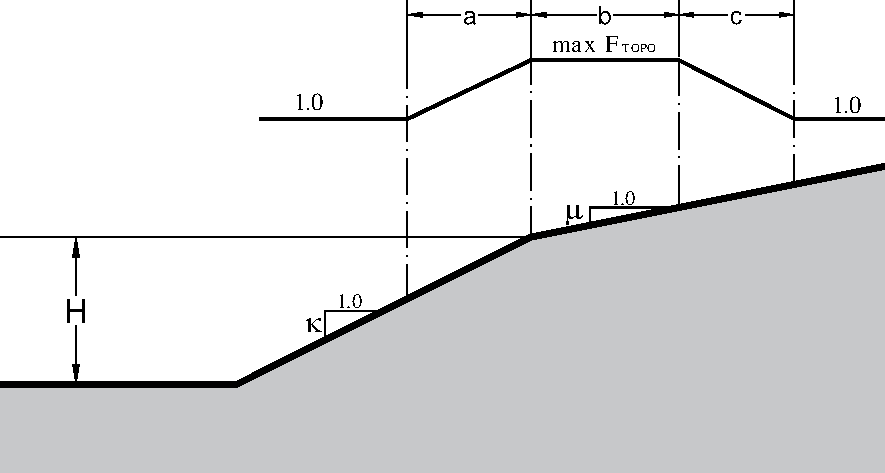
\includegraphics[width=10 cm]{img/AFPS_French_Juan.pdf}
	\caption{Factor de Agaravamiento Topográfico, Provisiones Sísmicas Francesas}
	\label{fig:afps}
	\vspace{-1.5 cm}
\end{figure}
%
Donde:
%
\begin{align*}
	&a=\dfrac{H}{3}\\
	&b=min\left( \dfrac{H+10}{4}, 20 \kappa \right)\\
	&c=\dfrac{H}{4}\\
	&max\ F_{TOPO} = 1.0 + 0.80 \left( \kappa - \mu -0.40 \right)\\
	&1.00 \leq max\ F_{TOPO} \leq 1.40
\end{align*}
%
El factor de agravamiento topográfico, definido como $max\ F_{TOPO}$ en la \cref{fig:afps}, aplica en las zonas definidas como \textit{a}, \textit{b} y \textit{c} en la parte superior de la \cref{fig:afps}. En la zona \textit{a}, el factor varía desde $1.0$ al lado izquierdo del vértice superior del talud hasta el valor máximo $max\ F_{TOPO}$ en el vértice superior. En la zona \textit{b}, el factor es constante sobre toda la zona e igual a $max\ F_{TOPO}$. En la zona \textit{c}, el factor varía desde el valor máximo $max\ F_{TOPO}$ hasta $1.0$ donde termina la zona \textit{c}. La variación del factor de agravamiento topográfico en las zonas \textit{a} y \textit{c} es lineal. Para inclinaciones menores a $22^{\circ}$, se desprecia el efecto topográfico.

En el \citeauthor{EC8} (\citeyear{EC8}), al igual que en la \citeauthor{AFPS1995}, se define un factor de agravamiento topográfico para geometrías como las mostradas en la \cref{fig:ec8}. En este caso, el factor de agravamiento varia de $1.00$ en la base de las geometrías hasta llegar a un valor máximo $max\ F_{TOPO}$, el cual depende de la inclinación del talud y del tipo de geometría, en la parte superior de la irregularidad geométrica.
%
\begin{figure}[H]
	\centering
	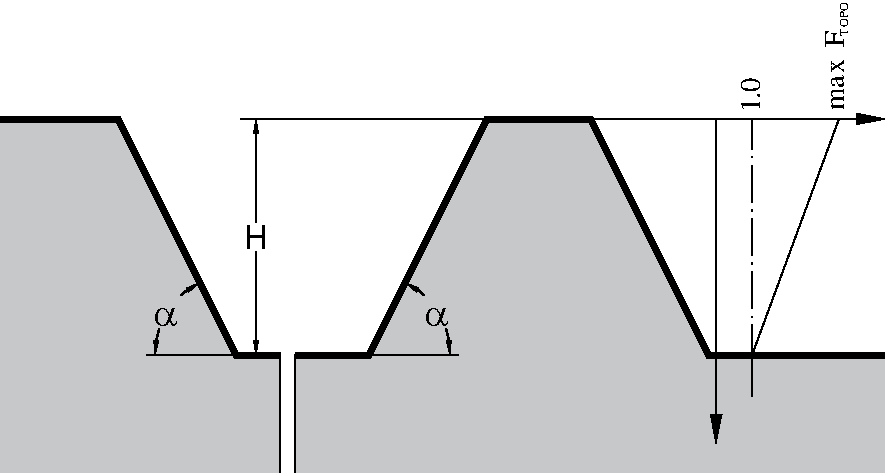
\includegraphics[width=10 cm]{img/EC8_Juan.pdf}
	\caption{Factor de Agaravamiento Topográfico, EuroCódigo}
	\label{fig:ec8}
%	\vspace{-1.5 cm}
\end{figure}
%
A continuación se presentan los valores límites del factor de agravamiento topográfico del \citeauthor{EC8}. Para el caso del talud aislado, el factor de agravamiento topográfico tiene un valor máximo $max\ F_{TOPO}=1.20$; este valor máximo aplica en la parte superior de la geometría en una distancia igual a la altura del talud. Para la geometría tipo talud, en la cual el ancho superior debe ser menor a la altura $H$, con $H>30 m$ y con inclinación entre $15^{\circ}$ y $30^{\circ}$, $max\ F_{TOPO}=1.20$; para inclinación mayor a $30^{\circ}$, $max\ F_{TOPO}=1.40$. 
%
\begin{align*}
&max\ F_{TOPO} =
  \begin{cases}
	1.40 \text{,} &  \alpha > 30^{\circ} \\
	1.20 \text{,} &  15^{\circ} \leq \alpha \leq 30^{\circ} \\
	1.00 \text{,} &  H<30 m\ \text{o}\  \alpha < 15^{\circ} \\
  \end{cases}
\end{align*}
%
Para ilustrar la aplicación de los factores de agravamiento topográfico, a continuación se presenta un ejemplo de aplicación, pero sobre un espectro de diseño obtenido a partir de la \citeauthor{NSR-10}, \citeyear{NSR-10}.\\
%
Para este ejemplo se definen los siguientes valores, a la luz de la \citeauthor{NSR-10}, \citeyear{NSR-10}. En la \cref{fig:nsr10} se muestra el espectro de diseño definido en la \citeauthor{NSR-10}.
%
\begin{itemize}
%
	\item[1.] Coeficiente de importancia, $I=1.0$ \vspace{-.5 cm}
	%
	\item[2.] Coeficiente de aceleración pico efectiva, $A_a=0.15$\vspace{-.5 cm}
	%
	\item[3.] Coefciente de velocidad pico efectiva, $A_v=0.20$\vspace{-.5 cm}
	%
	\item[4.] Perfil de suelo tipo \textit{D}
%
\end{itemize}
%
\begin{figure}[H]
	\centering
	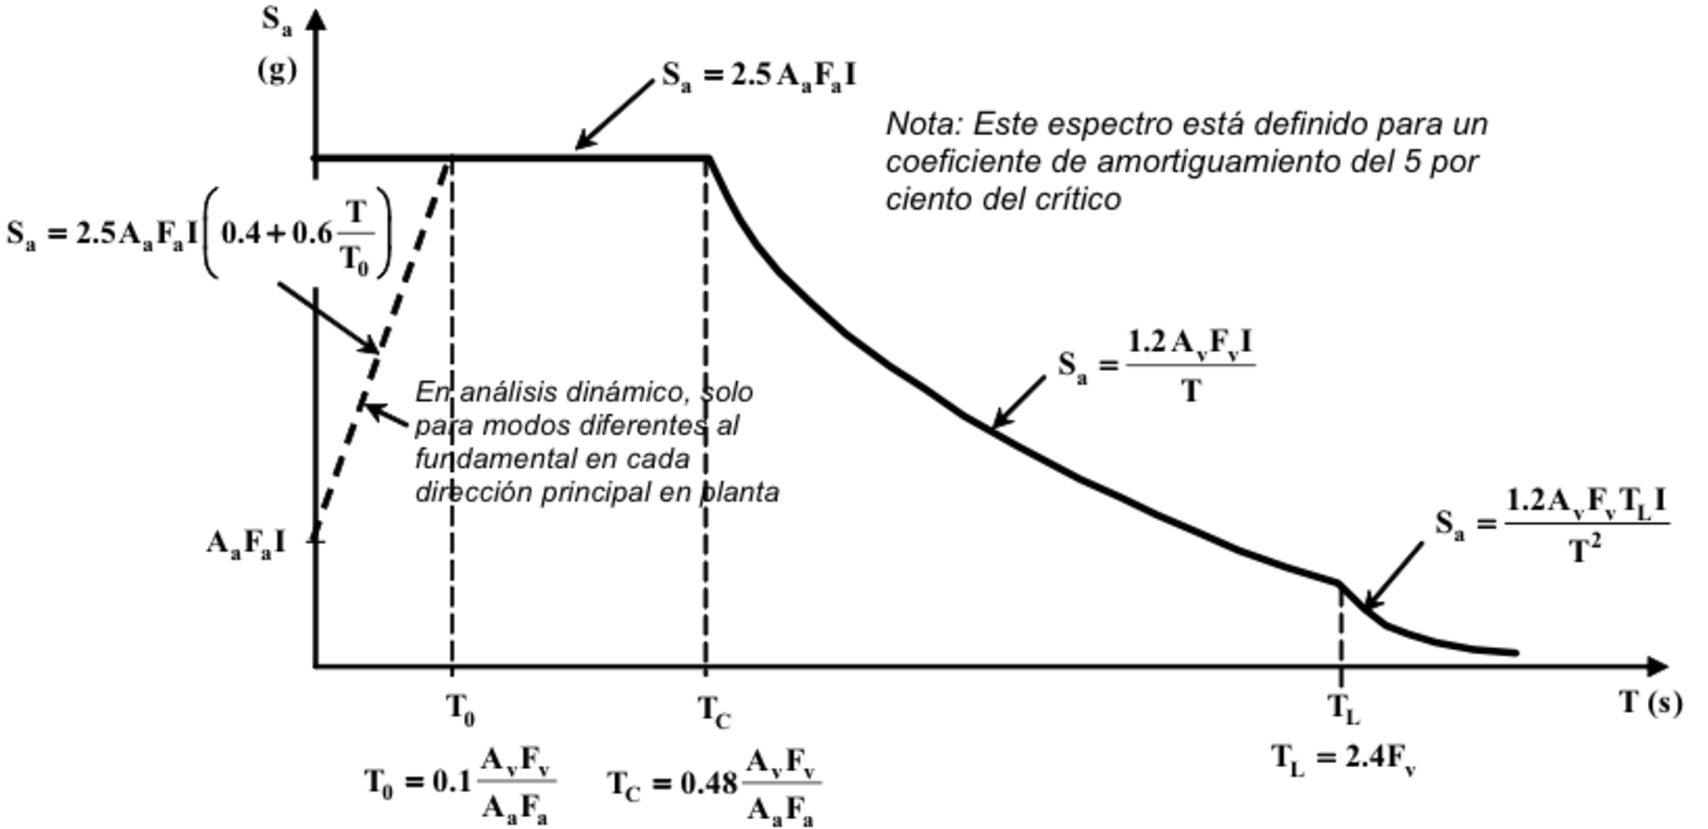
\includegraphics[width=12 cm]{img/EspectroNSR10.pdf}
	\caption{Espectro de Diseño, \citep[][Figura A.2.6-1]{NSR-10}}
	\label{fig:nsr10}
%	\vspace{-1.5 cm}
\end{figure}

%
En la \cref{fig:espmitlad} y \cref{fig:espcor} se presentan los espectros de diseño a la luz de la \citeauthor{NSR-10} \citeyear{NSR-10}, en esta mismas figuras se presentan estos espectros de diseño modificados por el factor de agravamiento topográfico definido en \citeauthor{AFPS1995} y \citeauthor{EC8}, sobre dos ubicaciones diferentes.

La \cref{fig:espmitlad} corresponde al espectro de diseño calculado sobre la mitad de la zona \textit{a}, según la \cref{fig:afps}. Para el caso de la norma \citeauthor{AFPS1995}, $max\ F_{TOPO} = 1.20$; para el \citeauthor{EC8}, $max\ F_{TOPO}=1.17$.
%
\begin{figure}[H]
	\centering
	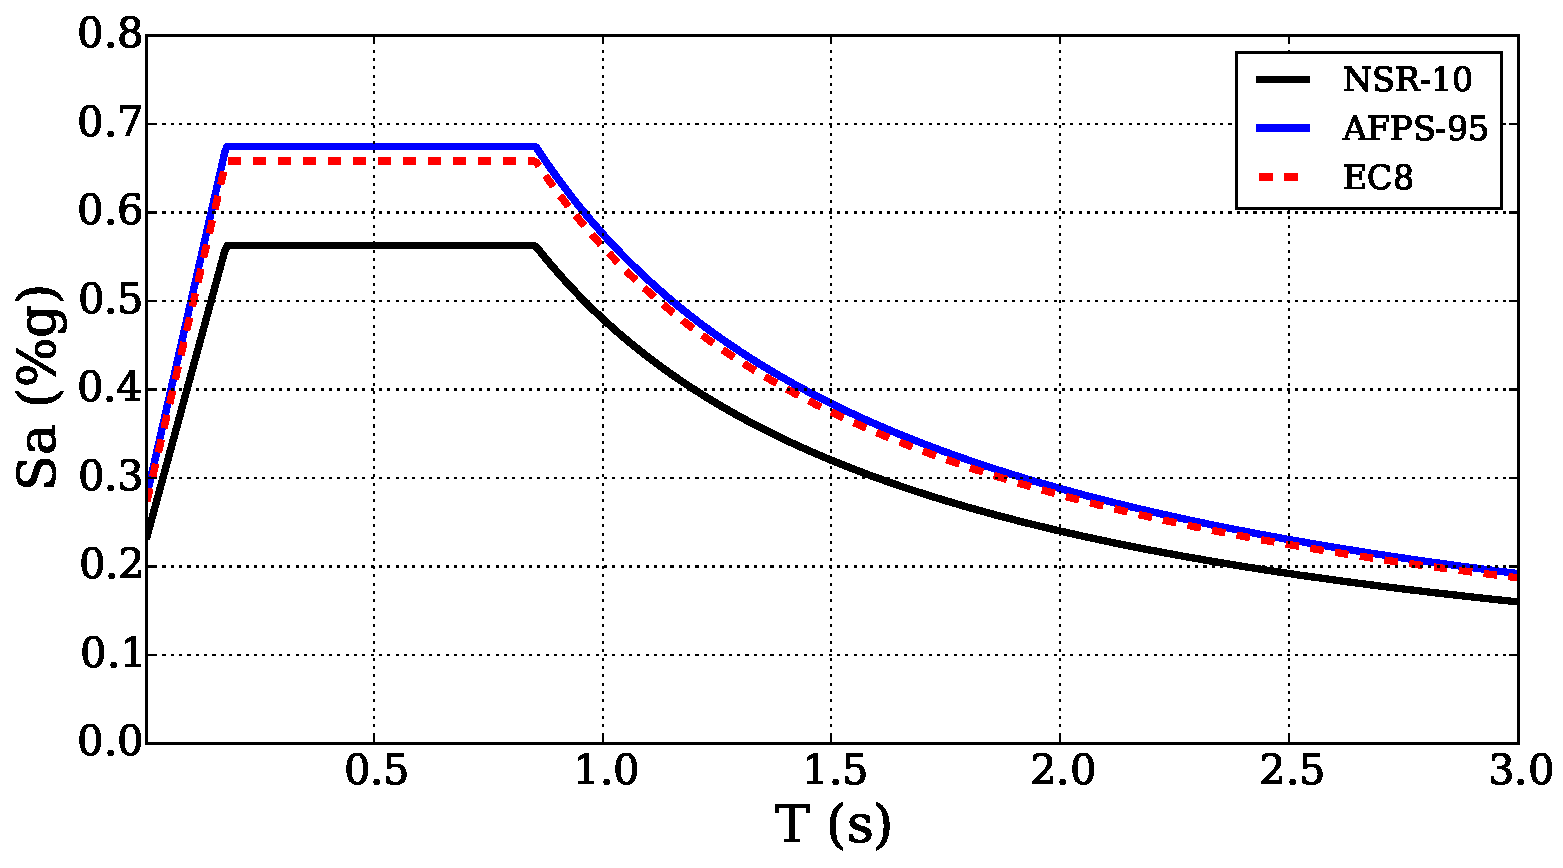
\includegraphics[width=10 cm]{img/EspectroZonaA.pdf}
	\vspace{-.5 cm}
	\caption{Espectro de Diseño Mitad Zona A}
	\label{fig:espmitlad}
%	\vspace{-1.5 cm}
\end{figure}
%
La \cref{fig:espcor} corresponde al espectro de diseño calculado sobre la zona \textit{b}, según la \cref{fig:afps}. Para la \citeauthor{AFPS1995} $max\ F_{TOPO}=1.40$ y para el \citeauthor{EC8} $max\ F_{TOPO}=1.20$.
%
\begin{figure}[H]
	\centering
	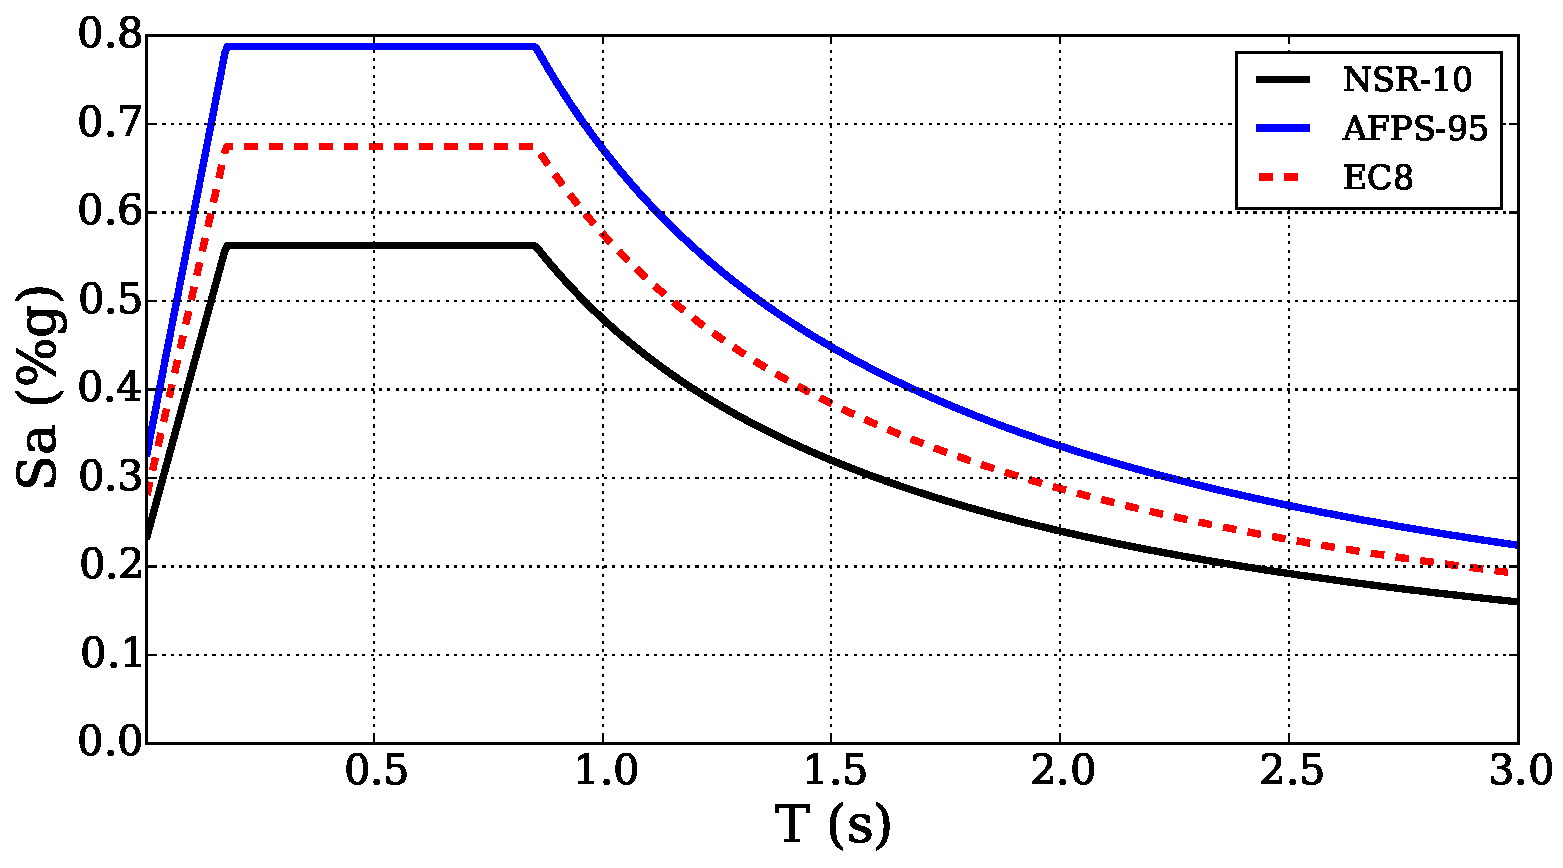
\includegraphics[width=10 cm]{img/EspectroZonaB.pdf}
	\vspace{-.5 cm}
	\caption{Espectro de Diseño Zona B}
	\label{fig:espcor}
%	\vspace{-1.5 cm}
\end{figure}
%
Para el caso del espectro de diseño calculado sobre la mitad de la zona A, la diferencia entre la norma \citeauthor{AFPS1995} y \citeauthor{EC8} se debe al hecho de que en el EuroCódigo la variación del factor de agravamiento se da desde la base del talud. En la corona, al menos dentro de la zona B, ambos factores son iguales al valor máximo probable definido para el factor de agravamiento topográfico definido en cada una de las normas.
%
\begin{figure}[H]
	\centering
	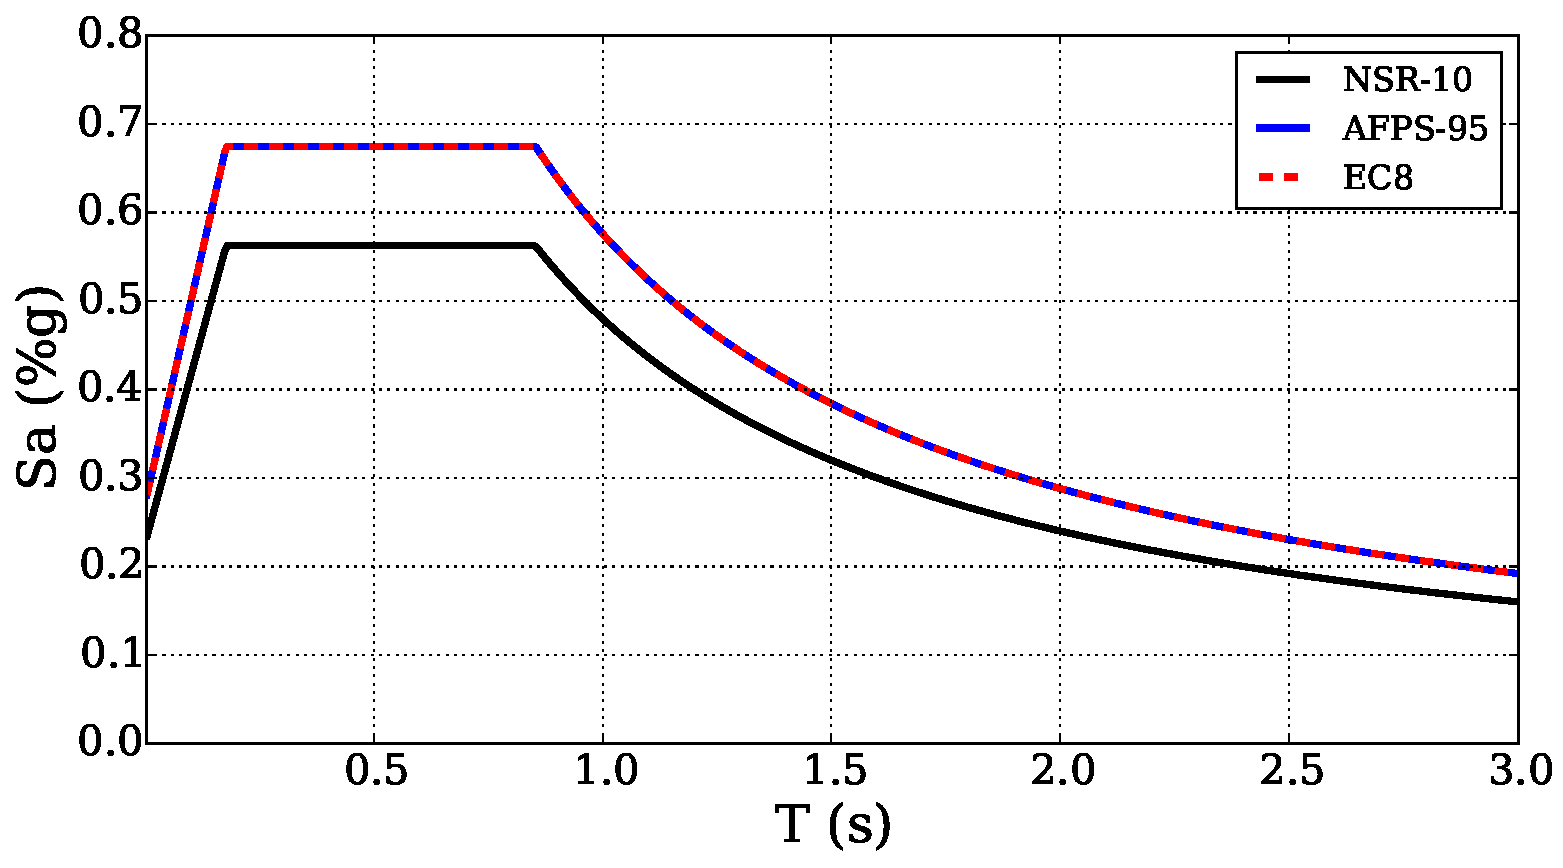
\includegraphics[width=10 cm]{img/EspectroZonaC.pdf}
	\vspace{-.5 cm}
	\caption{Espectro de Diseño Mitad Zona C}
	\label{fig:espzonc}
%	\vspace{-1.5 cm}
\end{figure}
%
En la \cref{fig:espzonc} se presenta el espectro de diseño calculado sobre la mitad de la zona C. Mientras el factor de agravamiento del \citeauthor{EC8} se mantiene constante sobre la corona de talud, el factor de la \citeauthor{AFPS1995} varia desde su máximo hasta su mínimo dentro de la zona C.

\textbf{Acá quiero poner el resultado de uno de los morros de Susana. Genero unos espectros, comparo con semiespacio y modificados por el factor de agravamiento topográfico del \citeauthor{EC8}, con el cual puedo comparar directamente.}
%
%
%
%
%
\newpage
%
\section{Superposición Basada en Difracción (SBD)}
\label{sbd}
%
En esta sección se presenta el Método de Superposición Basada en Difracción (SBD), presentado por \citeauthor{Jaramillo2013} (\citeyear{Jaramillo2013}), del cual los autores de esta propuesta son coautores. La importancia del método SBD para el desarrollo del presente trabajo radica en que este será utilizado para el análisis de las topografías regionales, tanto para estudiar la respuesta como para la interpretación de los resultados.

Inspirados en el trabajo de \citeauthor{Pathak1974} (\citeyear{Pathak1974}) y en el principio de superpocición, se desarrolla el método Superposición Basada en Difracción (SBD) para encontrar la solución completa al problema de propagación de frentes de ondas planos y cilíndricos tipo \textit{SH} incidiendo sobre topografías arbitrarias.

Son pocas las soluciones análiticas para problemas de elastodinámica las que se encuentran reportadas en la literetura \citep[por ejemplo][entre otras pocas]{SanchezSesma1990, SanchezSesma1985, Pathak1974, Trifunac1973, Tsaur2008, Tsaur2010a, Tsaur2010b, Han2011, Zhang2012a, Zhang2012b, Gao2012, Tsaur2013, Chang2013}, las cuales corresponden a la solución de casos altamente simplificados de propagación de ondas tipo \textit{SH}. Todas estas soluciones se presentan en términos de sumatorias infinitas, en las cuales la precisión está fuertemente influenciada por el número de términos que se usen en las sumatorias, las cuales muchas veces presentan problemas ya que estas emplean funciones con convergencia no uniforme. En el método SBD, la solución se construye progresivamente dependiendo de la precisión que se requiera alcanzar, basados en argumentos físicos, lo cual lo convierte en una gran herramienta para validación de simulaciones numéricas ya que es posible usarlo para la interpretación de resultados de modelos complejos. En el SBD, se usa una partición del campo total $u^T$, el cual se construye como la suma de un campo óptico o físico $u^o_P$ más un campo difractado $u^D$ \citep{Gomez2013}. El campo óptico se calcula de forma exacta a partir de las leyes de reflexión, mientras que el campo difractado se calcula aproximadamente a partir de las fuentes de difracción presentes en la topografía.
%
\begin{equation} u^T = u^o_P + u^D \label{eq:totalfield} \end{equation}
%
En la \cref{eq:totalfield}, el campo total se construye con el campo óptico o incoming físico, el cual corresponde a la suma del frente incidente $u^i$ más las reflexiones $u^r$ que se producen sobre la superficie libre, \cref{eq:optical}.
%
\begin{equation} u^o_P = u^i+ u^r \label{eq:optical}\end{equation}
%
Por su parte, el campo difractado, el cual se genera por la interacción de un frente de onda plano o cilíndrico con una singularidad geométrica, se calcula a partir de la solución presentada por \citeauthor{Pathak1974} (\citeyear{Pathak1974}). En este, se resuelve el problema de la incidencia de un frente de onda electromagnético, plano o cilíndrico, sobre una cuña infinta (\cref{fig:gendif}) haciendo uso de la teoría geométrica de la difracción propuesta por \citeauthor{Keller1962} (\citeyear{Keller1962}). La solución de \citeauthor{Pathak1974} (\citeyear{Pathak1974}) es particularizada en \citeauthor{Jaramillo2013} (\citeyear{Jaramillo2013}) al caso escalar de ondas tipo \textit{SH}.
%
\begin{figure}[H]
	\centering
	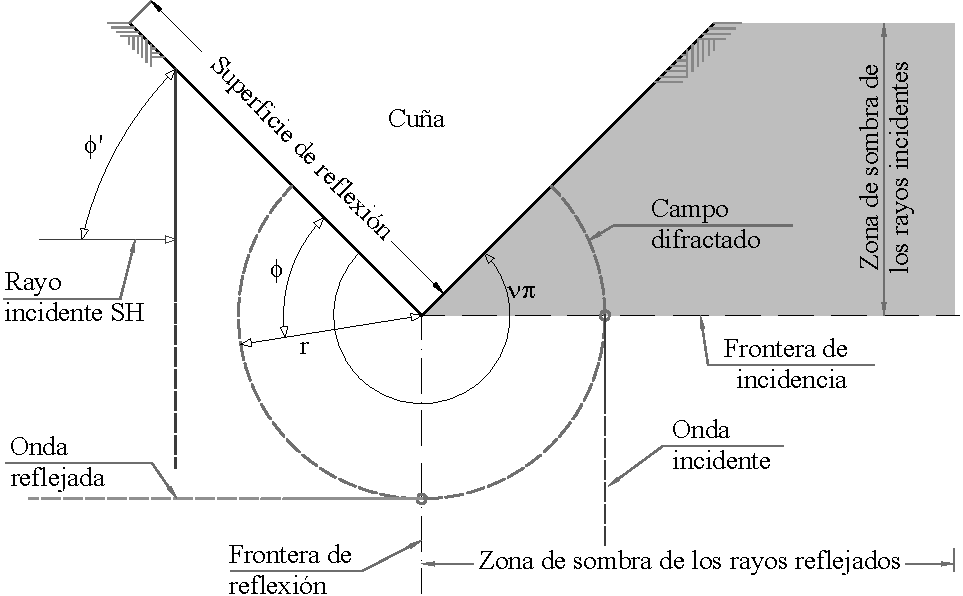
\includegraphics[width=10 cm]{img/GeneralDifraction.pdf}
	\caption{Campo difractado por una Cuña Infinita}
	\label{fig:gendif}
\end{figure}
%
En la \cref{fig:gendif} se presenta la cuña infinita usada para construir las topografías irregulares vía superposición. En esta se muestra la zona de sombra e iluminada del campo incidente y del reflejado.

En la \cref{eq:diffrac} se presenta la solución para el campo difractado, en la cual $r:$ es la coordenada radial desde el vértice de la cuña hasta el punto donde se quiere conocer el campo difractado, $\phi:$ coordenada angular del punto donde se quiere conocer el campo respecto a la frontera de reflexión, $\phi':$ ángulo de incidencia medido respecto a la frontera de reflexión, $\nu\pi:$ ángulo interno de la cuña (donde $\nu$ es un valor positivo que varía de $0.0$ a $2.0$), $r':$ radio de la onda cilíndrica incidente (áplica cuando incide un frente de onda cilíndrico), $k:$ número de onda y $\beta:$ corresponde a la velocidad de la onda incidente.
%
\begin{align}
w^{D}\left(\phi,r\right)&=A\frac{-e^{\left(-\hat{i}\left(kr+\pi/4\right)\right)}}{2\nu\sqrt{2\pi}\sqrt{kr}}\left[\cot\left(\frac{\pi+\left(\phi-\phi'\right)}{2\nu}\right)F\left(kLa^{+}\left(\phi-\phi'\right)\right)\right.\nonumber\\
&\left.+\cot\left(\frac{\pi-\left(\phi-\phi'\right)}{2\nu}\right)F\left(kLa^{-}\left(\phi-\phi'\right)\right)\right.\nonumber\\
&\left.+\cot\left(\frac{\pi+\left(\phi+\phi'\right)}{2\nu}\right)F\left(kLa^{+}\left(\phi+\phi'\right)\right)\right.\nonumber\\
&\left.+\cot\left(\frac{\pi-\left(\phi+\phi'\right)}{2\nu}\right)F\left(kLa^{-}\left(\phi+\phi'\right)\right) \right]
\label{eq:diffrac}
\end{align}
%
Los términos adicionales, presentados en la ecuación \ref{eq:diffrac}
\begin{align*}
&F\left(X\right)=2\hat{i}\sqrt{X}e^{\hat{i}X}
\int_{\sqrt{X}}^\infty e^{-\hat{i}\tau^2}\mathrm{d}\tau\\
&L=r\qquad\qquad\text{para onda plana incidente}\\
&L=\frac{rr'}{r+r'}\qquad\text{para onda incidente cilíndrica}\\
&a^{\pm}\left(\theta\right)=2\cos ^{2}\left(\frac{2\nu\pi N^\pm -\theta}{2}\right)\\
&N^+ =
  \begin{cases}
   0 & \text{if } \theta \leq \nu\pi -\pi \\
   1       & \text{if } \theta > \nu\pi -\pi
  \end{cases},\quad N^-=\begin{cases}
  -1 & \text{si } \theta < \pi -\nu\pi \\
   0 & \text{si } \pi -\nu\pi\leq \theta \leq \pi +\nu\pi \\
   1 & \text{si } \theta > \pi +\nu\pi
  \end{cases}
\end{align*}
%
Para ilustrar el método de superposición basado en difracción, se usa como caso de estudio el cañón en forma de $V$ presentado en la \cref{fig:canongen}. A continuación se presentan los pasos para construir la solución.
%
\begin{figure}[H]
	\centering
	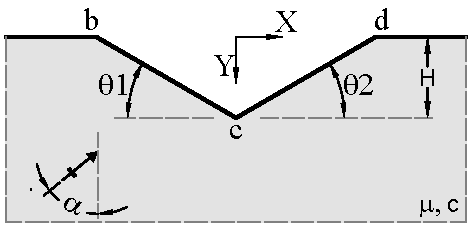
\includegraphics[width=10 cm]{img/vshaped1.pdf}
	\caption{Cañón utilizado para ilustrar el método de superposición basado en difracción (SBD).}
	\label{fig:canongen}
\end{figure}
%
%
%
%
%
\subsection{Construcción de la geometría superficial}
%
Para construir la geometría del cañón de la \cref{fig:canongen} se superponen varias cuñas fundamentales como la presentanda en la \cref{fig:gendif}. Cada una de las cuñas se describen a partir de dos parámetros, $\nu \pi$ y el ángulo de incidencia del frente de onda plano $\phi'$. Las cuñas usadas para construir la geometría aportan una parte del campo difractado, tanto difracciones de primer orden como de orden superior, el cual se encarga de restituir la continuidad del campo óptico y reconstruir el \textit{incoming} en el infinito.
%
\begin{figure}[H]
   \centering
    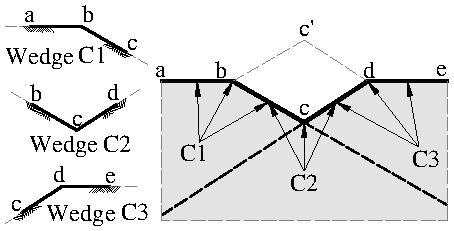
\includegraphics[width=10 cm]{img/vshapedw.pdf}
   \caption{Cañón generado a partir de la superposición de varias cuñas fundamentales.}
   \label{fig:canonsuper}
\end{figure}
%
Las cuñas necesarias para construir el cañón de la \cref{fig:canongen} se presentan en la \cref{fig:canonsuper}.
%
%
%
%
%
\subsection{Partición del dominio}
%
Para construir la respuesta total se procede realizando una partición del dominio. La primer partición se realiza sobre el campo óptico, considerando el campo incidente y las reflexiones que se generan sobre la superficie libre del dominio, ver \cref{fig:domrays}. Por ejemplo, en la \cref{fig:domrays} aparecen $6$ zonas con diferentes campos ópticos, zonas que se construyen a partir de la existencia o no de cada uno de los frentes que se muestran en la \cref{fig:domrays}. El campo incidente $R_1$, existe en todo el dominio, el campo reflejado sobre la superficie horizontal $R_2$ se propaga verticalmente hacia el interior del dominio, por último, los campos reflejados sobre las superficies inclinadas del dispersor se denotan como $R_3$ y $R_4$. Por ejemplo, la zona $5$ se genera con la suma de los frentes $R_1+R_2+R_3$
%
\begin{figure}[H]
    \centering
    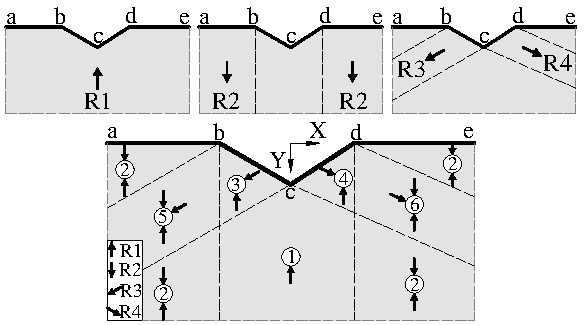
\includegraphics[width=10 cm]{img/dominiorays.pdf}
    \caption{Zonas del dominio con diferentes campos ópticos.}
    \label{fig:domrays}
\end{figure}
%
La segunda partición se realiza para encontrar el campo difractdo. En esta partición, se encuentran las zonas en las cuales existe campo difractado generado por cada una de los ápices de las cuñas con las que se construye el dispersor, \cref{fig:domdif} arriba. Superpuestas las zonas en las cuales se existe el campo difractado generado por cada cuña, se encuentran las regiones en las cuales el campo es diferente, \cref{fig:domdif} abajo. En la \cref{fig:domdif} se presentan las tres zonas en las cuales existen los diferentes campos difractados generados por el cañón de la \cref{fig:canonsuper}.\\
%
Los campos difractados generados por cada una de las cuñas se han nombrado $D_1$, $D_2$ y $D_3$. El campo difractado $D_2$ existe en todo el dominio de la \cref{fig:canonsuper}, mientras que los campos difractados $D_1$ y $D_2$ no, ya que estos solo existen en las zonas delimitadas por las lineas $a-b-g$ y $f-d-e$ respectivamente.
%
\begin{figure}[H]
    \centering
    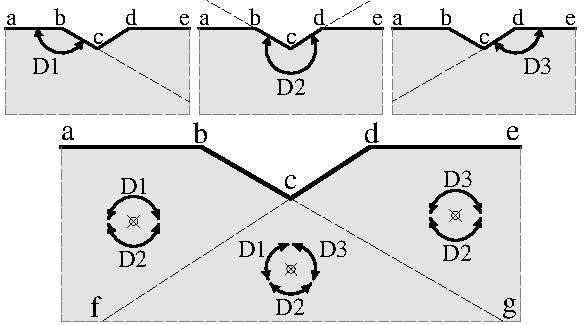
\includegraphics[width=10 cm]{img/dominiodif.pdf}
    \caption{Zonas del dominio con diferentes campos difractados.}
    \label{fig:domdif}
\end{figure}
%
%
%
%
%
\subsection{Difracción de orden superior}
%
Cuando un frente de onda difractado emana desde uno de los ápices de las cuñas, este se difracta nuevamente al alcanzar otro de los ápices, estos nuevos frentes los denominaremos difracciones de orden superior. Una difracción de primer orden será la originada por la interacción del frente incidente con uno de los ápices de las cuñas, el campo que esta difracción de primer orden genera al alcanzar otro ápice lo denominaremos difracción de segundo, y asi sucesivamente. El numero de ordenes de difracción a utilizar en la construcción de la respuesta total depende de la precisión que se quiera alcanzar.

Para evaluar una difracción de orden 2 o mayor, se utiliza nuevamente la \cref{eq:diffrac}, pero considerando el argumento para un frente de onda cilíndrico, ya que el campo difractado tiene dicha forma, teniendo el origen dicho campo difractado en la cuña que generó el campo a difractar.

Con referencia a la \cref{fig:domdif}, si se quiere conocer el campo difractado hasta orden 3, en la zona en la cual solo existen los campos $D_1$ y $D_2$, se emplea la \cref{eq:highorder}:
%
\begin{equation}
w^D=w^D_b+w^D_c+w^D_{b-c}+w^D_{c-b}+w^D_{d-c}+w^D_{b-c-b}+w^D_{c-b-c}+w^D_{d-c-b}+w^D_{c-d-c} 
\label{eq:highorder}
\end{equation}
%
Donde los subindices corresponden al ápice donde se ha difractad el campo. Por ejemplo, $w^D_b-c-b$ corresponde al frente incidente que primero es difractado en el ápice $b$, luego este frente difractado se difracta nuevamente en el ápice $c$ y por último en el ápice $b$.
%
%
%
%
%
\subsection{Campo total}
%
Para construir el campo total, es necesario sumar el campo óptico más el difractado en cada una de las zonas en las cuales se subdivide el dominio (\cref{fig:domrays} y \cref{fig:domdif}), superponiendo el campo óptico más el difractado.

En la zona 5, con referencia a la \cref{fig:domrays}, el campo total se construye como se muestra en la \cref{eq:total}, teniendo en cuenta solo tres ordenes de difracción.
%
\begin{eqnarray}
u^T=u^i+u^{R_1}+u^{R_2}+u^{R_3}+w^D_b+w^D_c+w^D_{b-c}+w^D_{c-b}+w^D_{d-c} \nonumber\\
+w^D_{b-c-b}+w^D_{c-b-c}+w^D_{d-c-b}+w^D_{c-d-c}
\label{eq:total}
\end{eqnarray}
%
En \cref{eq:total} $u^{R_i}$, corresponde al campo reflejado sobre la superficie libre del dominio \ref{fig:domrays}.
%
%
%
%
%
\subsection{Resultados}
%
Acá meteré los resultados que tenemos en el artículo del SBD.
%
%
%
%
%
\newpage
%
\section{Planteamiento del Problema}
%
En este proyecto vamos a estudiar el efecto de la topografía regional en la respuesta sísmica local, con el fin de incluirlo en el estudio de los efectos de sitio.

Los efectos de sitios, dentro de los cuales se encuentran la topografía y suelos locales, han sido identificados como los causantes de una fuerte modificación de la respuesta sísmica durante eventos sísmicos, causando una fuerte variación espacial de la respuesta con amplificaciones y deamplificaciones en sitios cercanos entre sí y generando una gran concentración de daño. Algunos ejemplos clásicos y recientes que ponen en evidencia la incidencia de los efectos de sitio en la respuesta local son las fuertes aceleraciones sobre la presa de Pacoima durante el sismo de San Fernando, California en 1971 \citep{trifunac1971analysis} donde se registraron aceleraciones iguales a $1.25g$ y sobre el distrito de Tarzana durante el sismo de Northridge, California 1994 \citep{spudich1996directional} donde el estudio del registro de las replicas mostró fuertes amplificaciones en la cima de una montaña respecto a la base de ésta, encontrandose factores entre $1.5$ y $4.5$ dependiendo de la componente del movimiento observado. Recientemente \citep{Assimaki2013}, continuando con el trabajo de \citep{Hough2011}, concluyen que la fuerte concentración de daño observado cerca del Hotel Montana, Haití, durante el sismo de magnitud Mw $7.0$ de 2010 se debió al acoplamiento de la topografía local y el suelo.

A pesar de que el problema de los efectos de sitio ha sido ampliamente estudiado durante las últimas décadas, la gran cantidad de variables involucradas en la determinación completa de estos hace que sea prácticamente imposible ponerlos en términos de unos factores simples de uso ingenieril dentro de normas de análisis y diseño sísmico, y la consideración de estos se limite al uso de modelos $1D$ de propagación de ondas, los cuales son una simplificación mayor.

Una alternativa bastante atractiva para estudiar la respuesta exacta de un sitio particular parece ser el uso de modelos a gran escala \citep[por ejemplo][]{Bielak2005, Lee2009a, Lee2009b, Ma2007, Cupillard2012} entre otros, los cuales son capaces de considerar los efectos de fuente, ruta de propagación, topografía local, tanto superficial como subsuperficial, y recientemente la topografía regional de forma exacta \citep{Doriam2014}. El uso de los modelos a gran escala requiere de estudios altamente detallados de los modelos de fuente y modelos de velocidad regional \footnote{\url{http://scec.usc.edu/scecpedia/CyberShake}}  \citep{Graves2011}, estudios que aún no cuentan con un consenso dentro de la comunidad cientifica, ya que los resultados pueden diferir altamente \footnote{\url{http://www.data.scec.org/research-tools/3d-velocity.html},\\	 \url{http://scec.usc.edu/scecpedia/CVM-S}} dependiendo de la técnica utilizada. Además, la implementación de estos modelos, por su complejidad y recursos necesarios, aún se encuentra lejos de poder ser usados por la comunidad ingenieríl en general.
%

Tradicionalmente, tal vez por la gran complejidad del problema, el estudio de los efectos de sitio para ser considerado en el diseño estructural, se basa en la suposición de que la respuesta de un sitio en particular se encuentra controlada por los espesores y propiedades mecánicas de los depósitos de suelos presentes y que estos depósitos se extienden infinitamente en la dirección horizontal con una altura constante, lo cual hace posible el uso de los modelos unidimenionales $\left( 1D \right)$ de propagación de ondas, sean éstas de corte \textit{S} o de cuerpo \textit{P}. Adicionalmente, estos modelos se basan o justifican en el hecho de que los sitios se encuentran lo suficientemente lejos de las fuentes para que en el viaje de las ondas desde ésta hasta el sitio, cambien su dirección y se propaguen verticalmente debido al efecto de la ley de Snell.\\
%
Estas hipótesis no tienen en cuenta el hecho de que la respuesta local se encuentra altamente influenciada por la topografía superficial y subsuperficial debido a que el problema se encuentra fuertemente acoplado. El no considerar el efecto acoplado suelo-topografía en la determinación de la respuesta local resulta en considerar movimientos de diseño bastante alejados de los reales, presentándose en algunos casos sobre-estimación y en otros sub-estimación de la respuesta.

Actualmente, los estudios de sitio se abordan por medio de microzonificaciones sísmicas, las cuales proporcionan espectros de respuesta de aceleraciones que aplican sobre pequeñas regiones, una ciudad puede ser dividida en muchas microzonas dependiendo del comportamiento mecánico de los suelos presentes en la región de estudio. Dichos estudios de microzonificación hacen uso de las \textit{Leyes de Atenuación o Ecuaciones de Predicción del Movimiento del Suelo} (\textit{GMPE} por sus siglas en ingles), las cuales se construyen a partir de los registros de las redes sismológicas nacionales, redes que se encuentran emplazadas a lo largo de todo un territorio nacional y ubicadas sobre roca para evitar que los registros se vean afectados por efectos mecánicos o topográficos. Con estos registros, junto con la sismologia regional, se generan curvas de amenaza uniforme en términos de taza de excedencia de aceleraciones para diferentes periodos de retorno. Es de suma importancia anotar que los registros de las redes sismológicas nacionales tienen en cuenta los efectos de fuente y ruta de propagación, y es por esta razón que los modelos uni-dimensionales $\left( 1D \right)$ también tienen en cuenta dichos efectos ya que estos se excitan con registros sintéticos generados a partir de las curvas de amenaza uniforme.

Sólo unas cuantas normas de análisis y diseño de estructuras sismorresistentes en el mundo \citep{EC8, AFPS1995}, especifican criterios para la consideración de los efectos de la topografía en la predicción de los movimientos del suelo, todas incluyen factores que tienen en cuenta el suelo local en función de la profundidad de los estratos y las velocidades de propagación de estos. Estas normas introducen factores de modificación espectral, conocidos como factores de agravamiento topográfico (FAT), los cuales son usados para modificar los espectros de diseño. Dichas funciones tienen varias deficiencias conceptuales, pues consideran que los efectos mecánicos y topográficos se encuentran desacoplados, y usan un factor de agravamiento topográfico constante para todo el espectro y son limitados en las geometrías consideradas.

En el presente trabajo vamos a distinguir dos tipos de efectos, \textit{Respuesta Local} y \textit{Respuesta Regional}, los cuales dependen de las longitudes de onda que se estén analizando, o más bien la relación entre las longitudes de onda analizadas y las dimensiones características de las geometrías.

\begin{figure}[H]
	\centering
	\subfloat [Modelo Local]{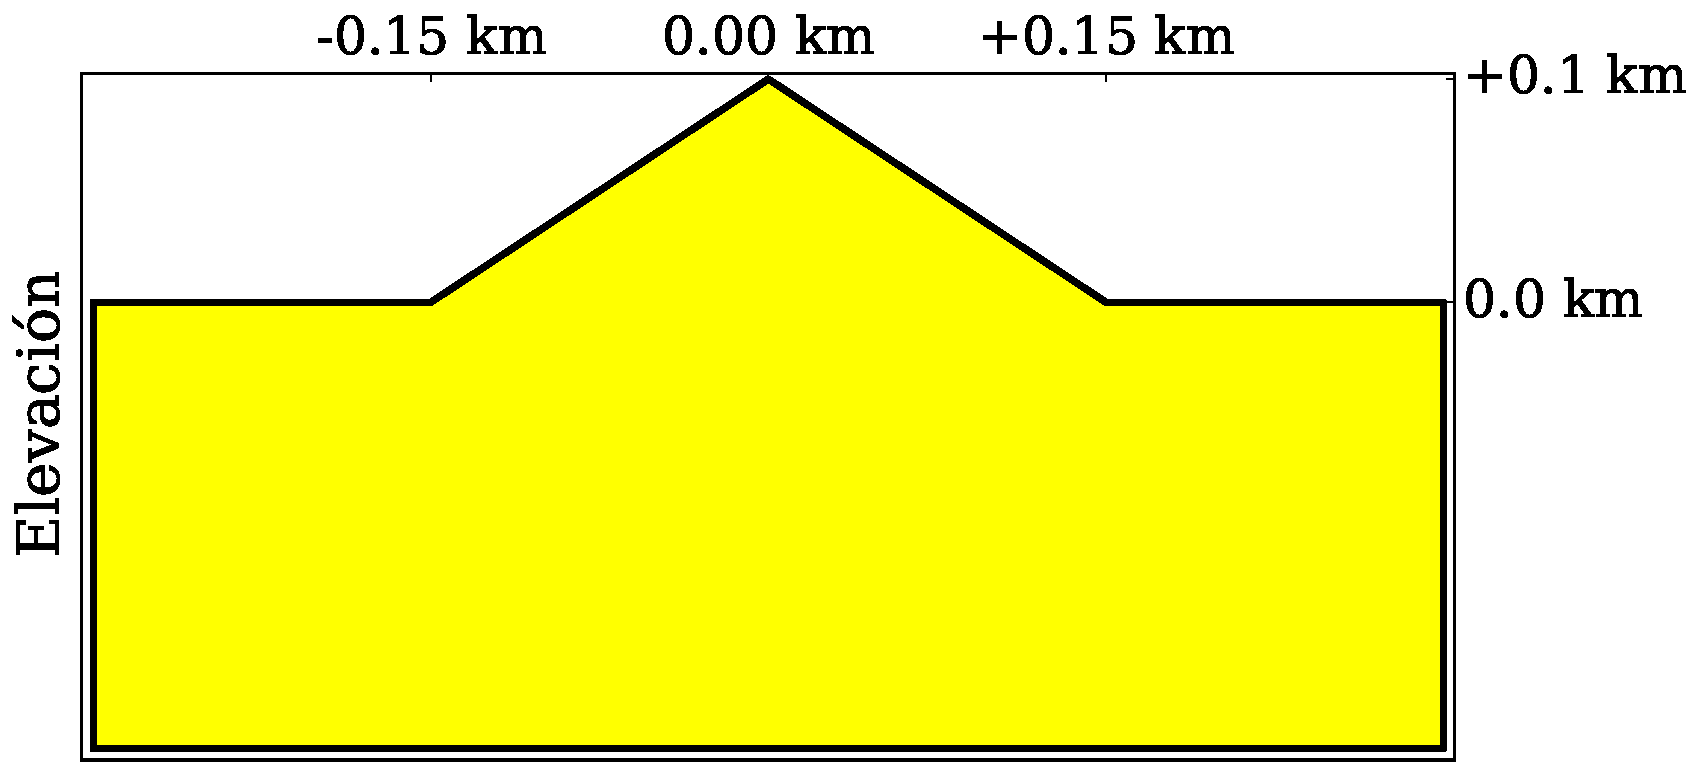
\includegraphics[width=8 cm]{img/ModelLocal.pdf}}
	%
	\subfloat [Modelo Regional]{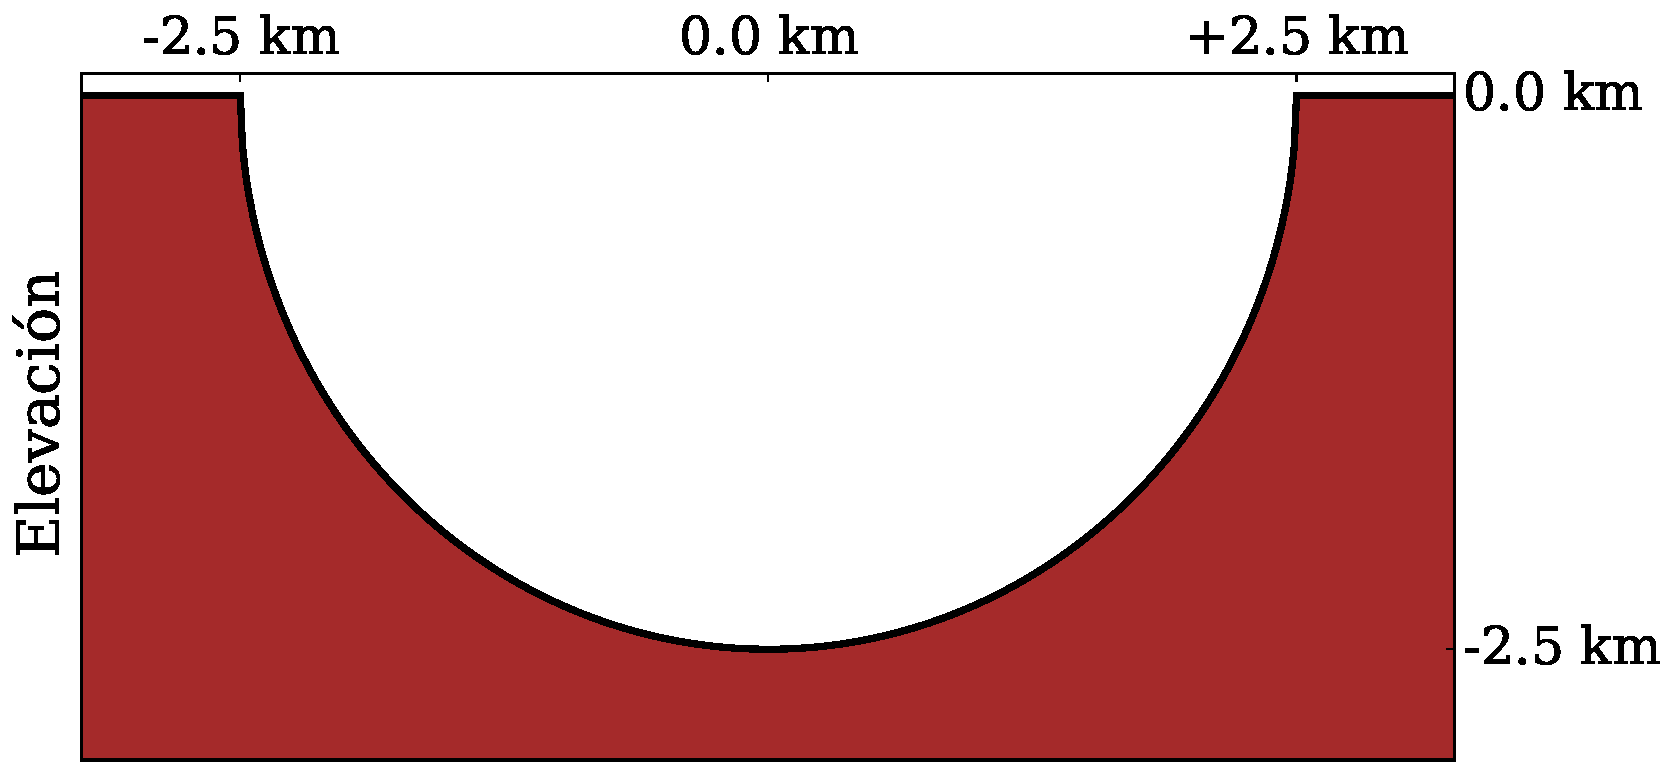
\includegraphics[width=8 cm]{img/ModelRegional.pdf}}
	\vspace{-.5 cm}
    \caption{Modelo local y regional.}
    \label{fig:modellocalregional}
    \vspace{-1 cm}
\end{figure}

La \cref{fig:modellocalregional} muestras dos geometrías con diferente orden de escala. La \cref{fig:modellocalregional}a corresponde al modelo de un dispersor tipo montaña, el cual dadas sus dimensiones, lo denominaremos \textit{Modelo Local} y al dispersor de la \cref{fig:modellocalregional}b, el cual corresponde a un cañón semicircular de radio $r=2.5\ km$, lo denominaremos \textit{Modelo Regional}. Ambos modelos son lineales, elásticos y homogéneos, con velocidad de propagación y densidad unitarias y se excitan con ondas de corte tipo \textit{SH}.

Para graficar las funciones de transferencia se usará la frecuencia adimensional $\eta$, la cual se define en la ecuación \cref{eq:eta} como:
%
%\begin{large}
	\begin{align}\label{eq:eta}
		\eta = \dfrac{b f}{\beta}
	\end{align}
%\end{large}
%
Donde $\beta$ corresponde a la velocidad de propagación de la onda de corte del dispersor (montaña), $f$ a la frecuencia de la excitación y $b$ al ancho de la montaña.

\subsection{Respuesta Local}

La respuesta local corresponde a la generada por topografías con dimensiones menores o iguales a $\ell$, geometría que no perturba la respuesta para longitudes de onda mucho mayores a dicha dimensión $\left( \lambda \gg \ell \right)$, dónde $\lambda$ es la longitud de onda, o que la perturbación que éstas generan en la respuesta es pequeña, comparada con la del semiespacio, y por ende es posible despreciarla.

\begin{figure}[H]
	\centering
	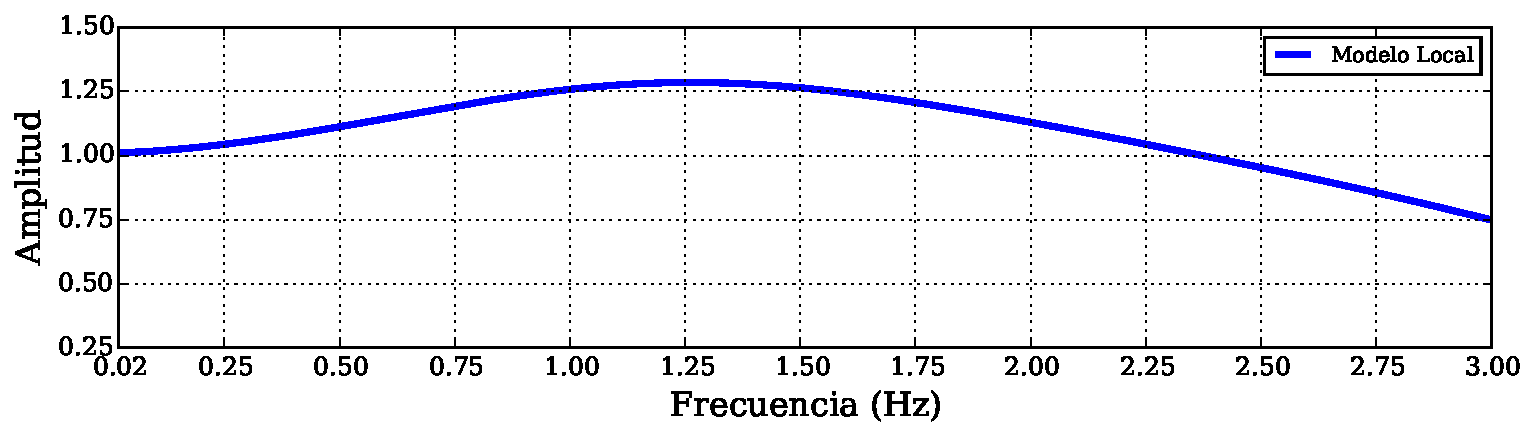
\includegraphics[width=15.5 cm]{img/LocalResponse.pdf}
	\vspace{-1 cm}	
	\caption{Función de Transferencia Modelo Local, Mitad Talud Izquierdo}
	\label{fig:localresponse}
	\vspace{-.5 cm}
\end{figure}

En la \cref{fig:localresponse} se presenta la función de transferencia sobre la mitad del talud izquierdo del dispersor de la \cref{fig:modellocalregional}a. En dicha figura se observa como para un rango de frecuencias bajo, longitud de onda mucho mayor que la base de la montaña analizada $\left( \lambda \gg base \right)$, la función de transferencia es muy cercana a la unidad $\left( FT\sim 1.0 \right)$, lo cual quiere decir que dicho dispersor no modifica, o lo hace muy poco, la respuesta. Es precisamente para dispersores con dimensiones que no exciten dichos rangos de frecuencias, que definiremos la \textit{Respuesta Local}.

\subsection{Respuesta Regional}

La respuesta regional corresponde a la generada por topografías con dimensiones mayores a $L$, dimensión que no modifica la respuesta para longitudes de onda lo suficientemente pequeñas $\left( \lambda \ll L \right)$ ya que éstas verán la geometría como un semiespacio y por tanto la función de transferencia tiende a la unidad $\left( FT \sim 1.0 \right)$.

\begin{figure}[H]
	\centering
	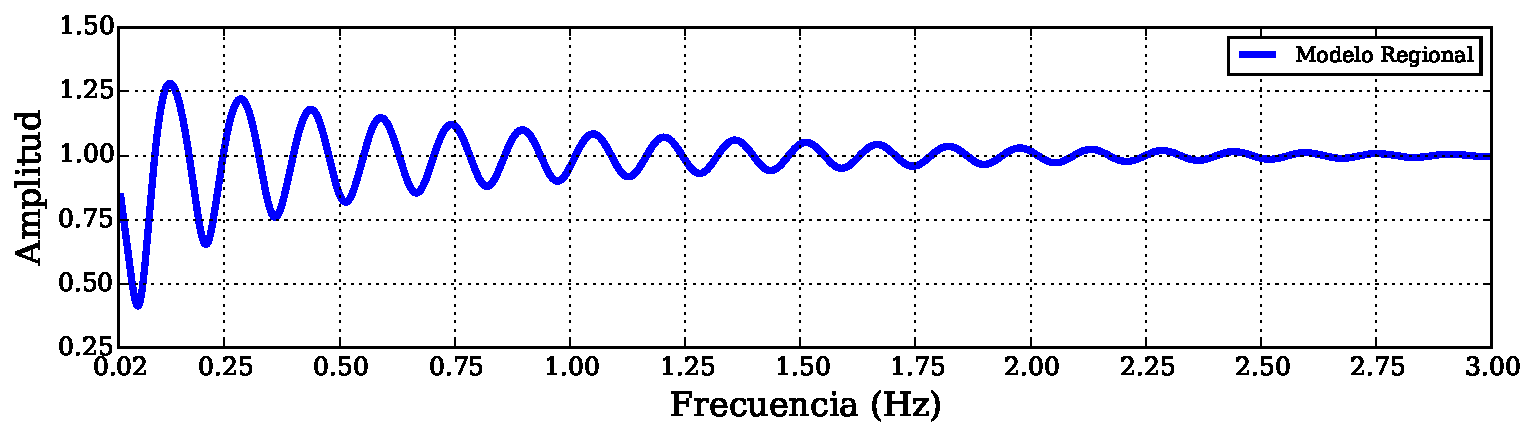
\includegraphics[width=15.5 cm]{img/RegionalResponse.pdf}
	\vspace{-1 cm}
	\caption{Función de Transferencia Modelo Regional Fondo del Cañón}
	\label{fig:regionalresponse}
	\vspace{-1 cm}
\end{figure}

En la \cref{fig:regionalresponse} se presenta la función de transferencia para un punto ubicado en el fondo del cañón semicircular del modelo regional, \cref{fig:modellocalregional}b. En dicha figura se observa como en la baja frecuencia, longitudes de onda grandes, la respuesta se aleja de la unidad, algunas veces amplificándose la respuesta y en otras deamplificándose, pero a partir de un rango de frecuencias determinado, la respuesta comienza a oscilar muy cerca de la unidad hasta que dicha oscilación se desvanece. Este tipo de respuestas, o geometrías a gran escala, serán las que denominaremos \textit{Respuesta Regional} ya que no modifica, o lo hace muy poco, la respuesta en la alta frecuencia.
%
%
%
%
%
\newpage
%
\section{Objetivos}
%
\subsection{Objetivo General}
%
Estudiar la incidencia de la topografía regional en la respuesta sísmica local.
%
\subsection{Objetivos Específicos}
%
\begin{itemize}
%
	%
	\item Demostrar la importancia de la respuesta regional en la respuesta de una geometría local.
	%
	\item Determinar el efecto topográfico regional de una región específica e incluir su efecto en la respuesta sísmica local de un sitio particular.
	%
	\item Proponer una metodología para la elaboración de estudios de microzonificación sísmica considerando el efecto regional de la topografía y el efecto local acoplado suelo-topografía.
	%
	\item Tomar como base una microzonificación sísmica ficticia o existente, elaborada con los modelos tradicionales $1D$ de propagación de ondas, comparar los resultados versus la metodología propuesta para modelos $1D$, $2D$ y $3D$ de propagación de ondas.
%
\end{itemize}
%
%
%
%
%
\newpage
%
\section{Metodología}
\label{metodologia}
%
Para lograr el objetivo principal del presente trabajo, el cual consiste en calcular e incluir el efecto de la topografía regional en los estudios de efectos de sitio, es necesario que se cumplan las tres hipótesis fundamentales en las cuales nos basamos. Primero, la respuesta en la baja frecuencia se encuentra controlada por las topografías regionales, de gran escala. Segundo, la respuesta en la alta frecuencia se encuentra controlada por las geometrías locales. Por útlimo, es necesario demostrar que la respuesta total se puede construir como la superposición de una respuesta en la baja frecuencia, \textit{Respuesta Regional}; y una respuesta en la alta frecuencia, \textit{Respuesta Local}.

La metodología propuesta consiste en construir la respuesta total de un sitio particular como la superposición de una respuesta regional, debida a la topografía regional o de gran escala, y una respuesta local o de menor escala, debida a la topografía local y la estratigrafía del sitio. El efecto topográfico regional, el cual es el principal objetivo a estudiar dentro de este proyecto, será calculado a partir de modelos semi-analíticos o con simulaciones que solo capturen la respuesta en la baja frecuencia, ya que en la alta frecuencia la respuesta debe acercarse bastante a la de un semiespacio. La respuesta local se obtendrá a partir de simulaciones detalladas usando modelos computacionales con elementos finitos, asumiendo que estos se encuentran soportados sobre un semi-espacio lineal elástico, pero pudiéndose considerar el comportamiento no-lineal de los diferentes materiales locales. Los modelos locales podrán ser $1D$, $2D$ o $3D$. Los modelos computacionales por elementos finitos se excitarán usando los procedimientos convencionales para los modelos $1D$ de propagación de ondas; en los cuales un espectro de amenaza sísmica uniforme se convierte en una familia de acelerogramas sintéticos en roca, los cuales deben representar sismos generados por fuentes ubicadas a diferentes distancias de la región de estudio. A los acelerogramas sintéticos se les calculará los espectros de Fourier para modificarlos con las funciones de transferencia de la respuesta regional y nuevamente se llevarán al dominio del tiempo para tener así unos acelerogramas sintéticos que incluyan el efecto de la topografía regional. Estos acelerogramas sintéticos modificados por el efecto topográfico regional se aplicarán como excitación de los modelos computacionales del sitio, inicialmente en foma de ondas planas tipo $SH$ y $SV$ incidiendo verticalmente, y por último empleando modelos tridimensionales $\left( 3D \right)$.\\
%
Para el análisis de los modelos locales se desarrollará una herramienta computacional, la cual permitirá considerar el efecto acoplado suelo-topografía en el rango lineal y no-lineal. La herramienta computacional a desarrollar se encuentra basada en el método del dominio reducido, DRM por sus siglas en inglés, presentado por \citeauthor{bielak2003} (\citeyear{bielak2003}) para poder incluir los efectos de fuente en simulaciones a gran escala sobre escenarios reales. En nuestro trabajo utilizaremos una versión modifcada del DRM, ya que primero calcularemos la respuesta debida únicamente a la topografía regional, respuesta que usaremos para modificar la excitación de los modelos locales.

A continuación se presenta una descripción detallada de nuestra metodología, la cual según el conocimiento de los autores de esta propuesta no ha sido presentada antes:

Partiendo del espectro de amenaza uniforme $S_{a}^{UH} \left( T \right)$, el cual se calcula en roca y se encuentra libre de efectos mecánicos y topogáficos, es posible generar historias de aceleraciones sintéticas $a_{i}^{UH}\left( t \right)$. Es necesario generar varias señales, las cuales deben ser representativas de sismos ocurridos a diferentes distancias del sitio bajo estudio, donde cada señal genera un espectro de respuesta $S_{a}^{i} \left( T \right)$ diferente al de amenaza uniforme pero los cuales se encuentran contenidos dentro de este.

%\begin{align}
	$S_{a}^{UH} \left( T \right) \Rightarrow a_{i}^{UH}\left( t \right) \Rightarrow S_{a}^{i} \left( T \right)$
%\end{align}

Donde $S_{a}^{UH} \left( T \right)$ corresponde al espectro de respuesta de amenaza uniforme, $a_{i}^{UH}\left( t \right)$ $i$-esima señal sintética generada a partir del espectro de amenaza uniforme y $S_{a}^{i} \left( T \right)$ al espectro de respuesta de la $i$-esima señal sintética. Además se tiene que:
%
%\begin{large}
	\begin{align}
		S_{a}^{1} \left( T \right) \cup S_{a}^{2} \left( T \right) \cup S_{a}^{3} \left( T \right) \cup ... \cup S_{a}^{n} \left( T \right) = S_{a}^{UH} \left( T \right)
		\vspace{-1 cm}
	\end{align}	
%\end{large}
%
%
De las señales sintéticas es posible calcular el espectro de Fourier de cada una de ellas, teniendo en cuenta que éstas contienen el campo incidente y el reflejado:
%
%\begin{large}
	\begin{align}\label{eq:espfouhs}
		\widehat{A}^{HS}_{i} \left( \hat{i} \omega \right) = \dfrac{1}{2} \widehat{A}^{FS}_{i} \left( \hat{i} \omega \right)
	\vspace{-1 cm}
	\end{align}
%\end{large}
%
Donde $\widehat{A}^{FS}_{i} \left( \hat{i} \omega \right)$ corresponde al espectro de Fourier de la $i$-esima señal sintética, incluye el campo incidente y el reflejado, $\widehat{A}^{HS}_{i} \left( \hat{i} \omega \right)$ es el espectro de Fourier de la $i$-esima señal sintética, en esta sólo incluye el campo incidente.\\
%
El espectro de Fourier de la $i$-esima señal sintética se define como:
%
%\begin{large}
	\begin{align}\label{eq:fourdirec}
		\widehat{A}^{FS}_{i} \left( \hat{i} \omega \right) = \int_{-\infty}^{+\infty} a_{i}^{UH} \left( t \right) e^{-\hat{i} \omega t} dt 
	\vspace{-1 cm}
	\end{align}
%\end{large}
%
El proceso anterior se puede resumir en el siguiente esquema:

%\begin{large}
	$a_{i}^{UH}\left( t \right) \Rightarrow \widehat{A}^{FS}_{i} \left( \hat{i} \omega \right) \Rightarrow \widehat{A}^{HS}_{i} \left( \hat{i} \omega \right)$
%\end{large} 

Para calcular la respuesta de la topografía regional, la región bajo estudio se aproxima a una geometría sencilla, la cual puede ser posible estudiarla mediante procedimientos semi-analíticos o con simulaciones que solo incluyan la respuesta lineal en la baja frecuencia. En la \cref{fig:geolocreg} se presenta un ejemplo hipotético de una geometría regional en conjunto con la geometría aproximada; la geometría regional se muestran algunas geometrías locales y la presencia de diferentes materiales. En la geometría aproximada se ha homogeneizado el dominio, siendo esta homegenización una de la hipótesis fundamentales de esta propuesta, hipótesis que deberá ser justificada dentro del desarrollo del proyecto.
%
\begin{figure}[H]
	\centering
	\subfloat [Geometría Regional]{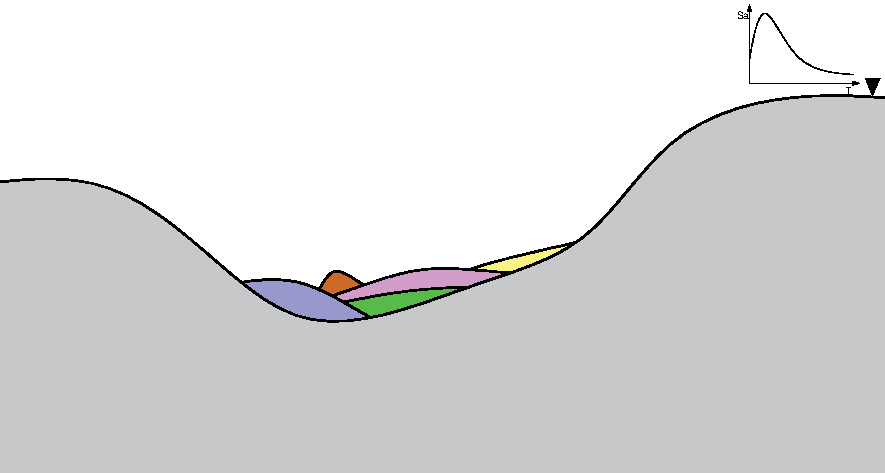
\includegraphics[width=7.5 cm]{img/Regional.pdf}}
	\hspace{.25 cm}
	\subfloat [Geometría Regional Aproximada]{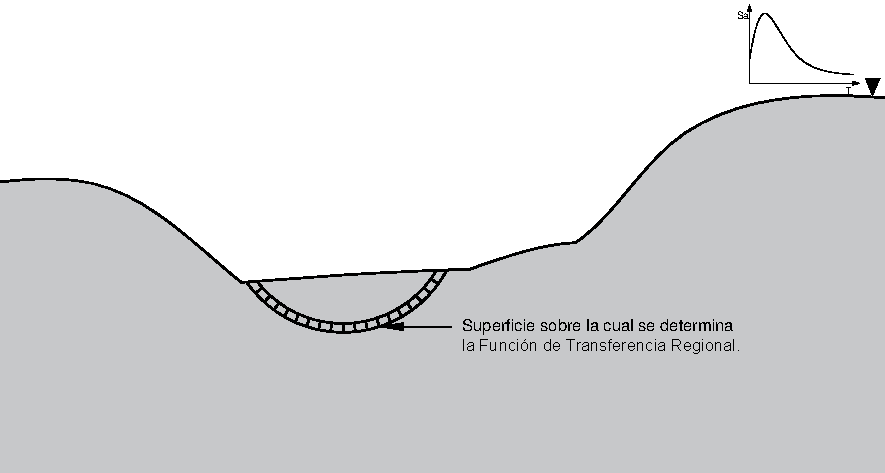
\includegraphics[width=7.5 cm]{img/FunTrans.pdf}}
	\vspace{-.5 cm}
    \caption{Geometría Regional.}
    \label{fig:geolocreg}
    \vspace{-1 cm}
\end{figure}
%
La respuesta de la topografía regional de la \cref{fig:geolocreg}b, en términos de funciones de transferencia $FT^{Reg} \left(\hat{i} \omega \right)$, se emplea para modificar los espectros de Fourier de las señales sintéticas.
%
%\begin{large}
	\begin{align}\label{eq:espfoumod}
		\widehat{A}^{Reg}_{i} \left( \hat{i} \omega \right) = \widehat{A}^{HS}_{i} \left( \hat{i} \omega \right) FT^{Reg} \left( \hat{i} \omega \right)
	\vspace{-1 cm}
	\end{align}
%\end{large}
%
Donde $\widehat{A}^{Reg}_{i} \left( \hat{i} \omega \right)$ corresponde al espectro de Fourier modificado por el efecto de la topografía regional. A partir del espectro de Fourier modificado se calculan las nuevas señales sintéticas vía la transformada inversa de Fourier, señales que se emplean para excitar los modelos locales.
%
%\begin{large}
	\begin{align}\label{eq:fourinv}
		a_{i}^{Reg} \left( t \right) = \dfrac{1}{2 \pi} \int_{-\infty}^{+\infty} \widehat{A}^{Mod}_{i} \left( \hat{i} \omega \right) e^{\hat{i} \omega t} d \omega
	\vspace{-1 cm}
	\end{align}
%\end{large}
%
El proceso anterior se puede resumir en el siguiente esquema:

%\begin{large}
	$FT^{Reg} \left( \hat{i} \omega \right) \Rightarrow \widehat{A}^{Reg}_{i} \left( \hat{i} \omega \right) \Rightarrow a_{i}^{Reg}\left( t \right)$
%\end{large}

Las señales sintéticas modificadas $a_{i}^{Reg}\left( t \right)$ se emplean para excitar los modelos locales, los cuales incluyen la topografía superficial y sub-superficial; pudiendo también ser estos modelos $1D$, pero diferenciandose de la metodología tradicional en el hecho de que la excitación de estos contiene el efecto de la topografía regional. La necesidad de considerar sismos que representen fuentes ubicadas a diferentes distancias del sitio de estudio se debe a que es necesario estudiar la respuesta lineal y no-lineal de los modelos.
%
\begin{figure}[H]
	\centering
	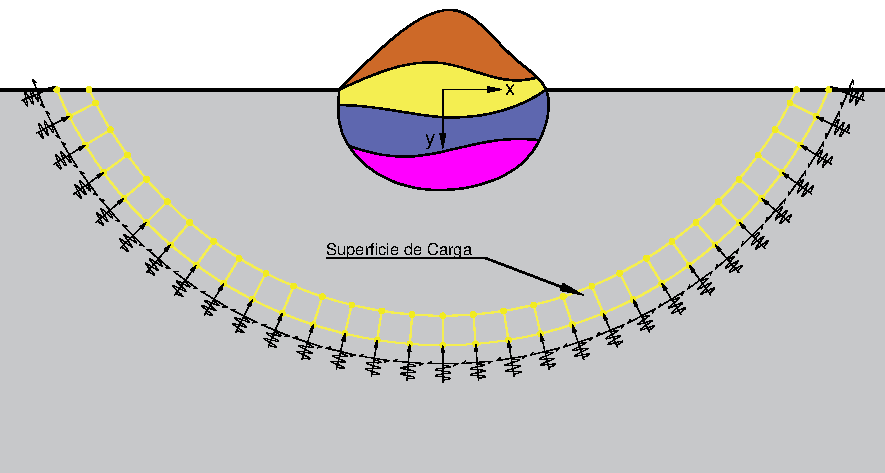
\includegraphics[width=12 cm]{img/Local.pdf}
	\vspace{-.5 cm}
	\caption{Modelo Local}
	\label{fig:local}
	\vspace{-1 cm}
\end{figure}
%
En la \cref{fig:local} se presenta el esquema de un modelo local, el cual contiene topografía superficial y subsuperficial, presencia de diferentes materiales, sobre un semiespacio homogéneo junto con la superficie sobre la cual se aplica la excitación modificada por los efectos regionales.

El análisis de los modelos locales es el encargado de capturar la respuesta en la alta frecuencia, respuesta generada por la topografía y el efecto mecánico local; el efecto acoplado suelo-topografía. La formulación aquí presentada es diferente a la original del DRM presentada por \citeauthor{bielak2003} (\citeyear{bielak2003}) ya que en la primer etapa calculamos la respuesta regional sin la topografía ni materiales locales, respuesta que posteriormente modifica el campo incidente y se aplica como una carga efectiva como se muestra en la \cref{fig:local}. El método para excitar los modelos locales se implementará en software comercial por elementos finitos de manera que pueda ser usado fácilmente en los estudios de efectos de sitio.

La respuesta de los modelos computacionales locales, en términos de aceleraciones, se usarán para calcular los espectros de respuesta totales $S_{a}^{Tot} \left( T \right)$, los cuales consideran los efectos de fuente y ruta de progagación, al ser estos excitados con señales sintéticas generadas a partir de espectros de amenaza uniforme $S_{a}^{UH} \left( T \right)$, el efecto de la topografía regional con la consideración de la función de transferencia regional $FT^{Reg} \left( \hat{i} \omega \right)$, y la respuesta lineal y no-lineal del efecto acoplado suelo topografía local.\\
%
Los espectros de respuesta totales $S_{a}^{i-Tot} \left( T \right)$, para cada una de las señales sintéticas y sobre toda la superficie del dominio, se usarán para calcular la relación de respuesta espectral, la cual se usa para modificar el espectro de amenaza uniforme por el efecto regional y acoplado suelo-topografía local.
%
%\begin{large}
	\begin{align}\label{eq:rrs}
		\mathcal{RRS}^{i} \left( T \right) = \dfrac{S_{a}^{i-Tot} \left( T \right)}{S_{a}^{i} \left( T \right)}
	\vspace{-1 cm}
	\end{align}
%\end{large}
%
%\begin{large}
	\begin{align}\label{eq:rrs}
		S_{a}^{UH-Reg} \left( T \right) = S_{a}^{UH} \left( T \right) * \text{envol} \left\lbrace \mathcal{RRS}^{i} \left( T \right) \right\rbrace
	\vspace{-1 cm}
	\end{align}
%\end{large}
%
Donde $S_{a}^{UH-Reg} \left( T \right)$ corresponde al espectro de amenaza uniforme modificado por el efecto regional y local, $\text{envol} \left\lbrace \mathcal{RRS}^{i} \left( T \right) \right\rbrace$ corresponde a la envolvente de las relaciones de respuestas espectrales.
%
%
%
%
%
\newpage
%
\section{Resultados Preliminares}
%
La metodología propuesta se emplea para analizar un modelo simplificado sobre el que incide verticalmente una onda plana tipo $SH$. Para el análisis de los modelos regionales y locales se utiliza un programa computacional de Elementos de Frontera 2D (BEM por sus siglas en inglés) desarrollado al interior del grupo de Mecánica Aplicada de la Universidad EAFIT (Medellín, Colombia), el cual encuentra la respuesta en el dominio de la frecuencia y por lo tanto los resultados se limitarán, en esta propuesta, al rango lineal. Todos lo cálculos fueron realizados en el computador de alto desempeño Apolo de la Universidad EAFIT.
%
\begin{figure}[H]
	\centering
	\subfloat [Modelo Completo]{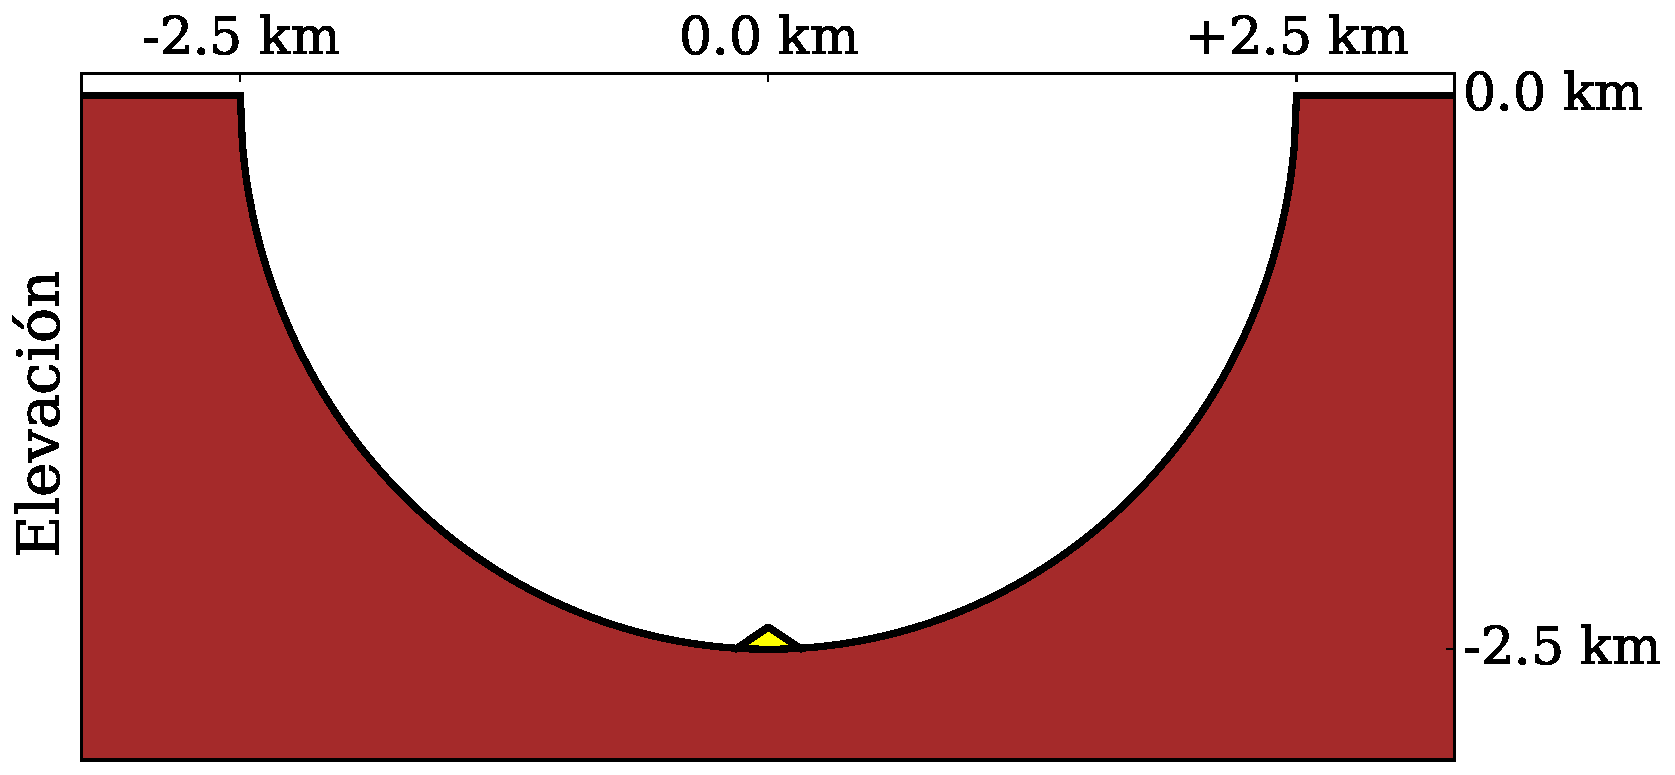
\includegraphics[width=16 cm]{img/ModelRegionalComplete.pdf}}\\
	%
	\subfloat [Modelo Local]{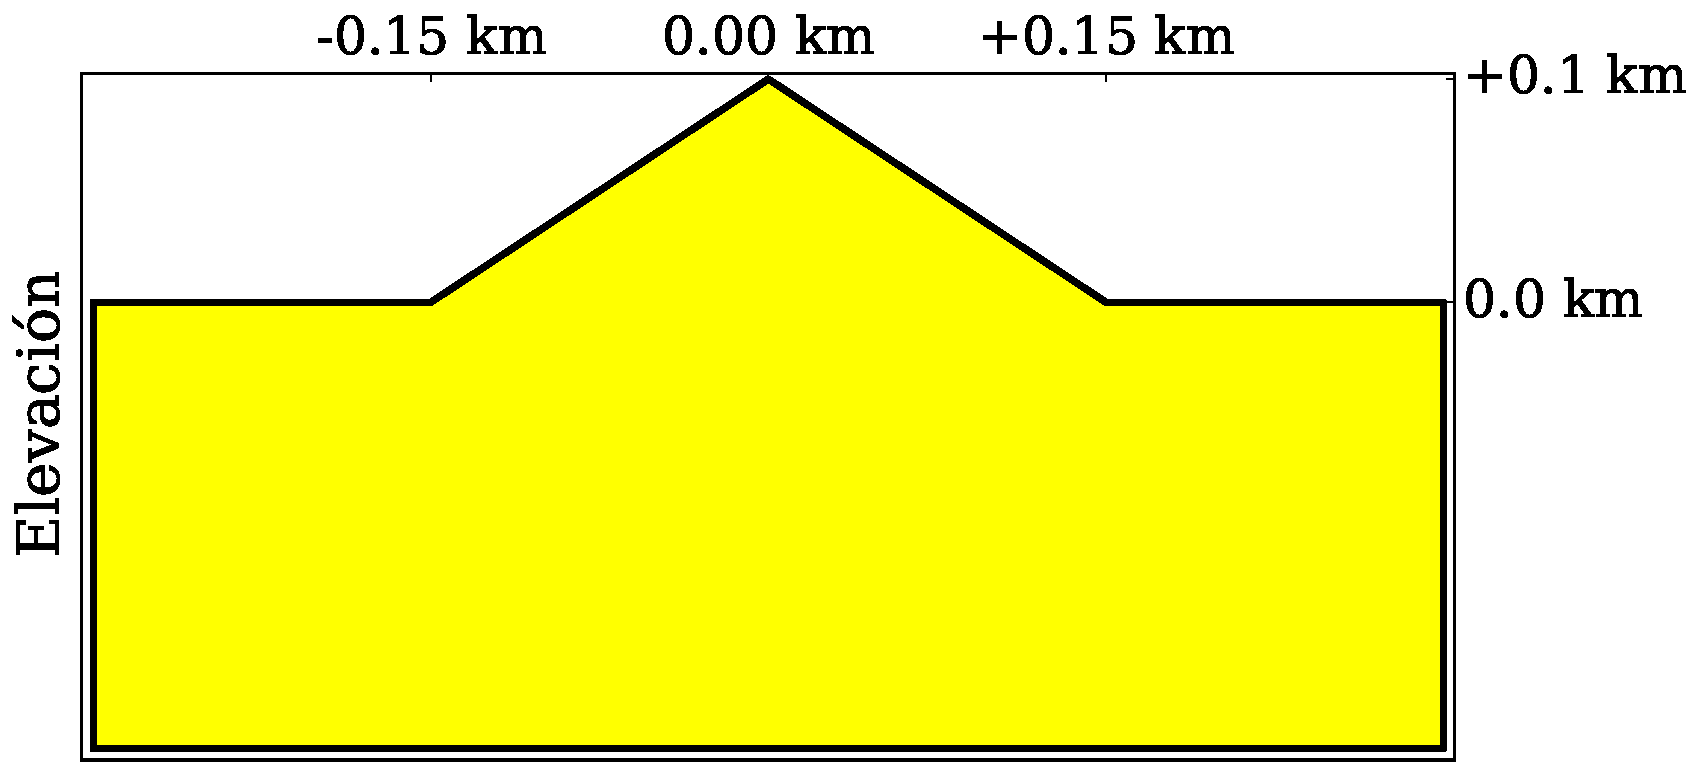
\includegraphics[width=8 cm]{img/ModelLocal.pdf}}
	%
	\subfloat [Modelo Regional]{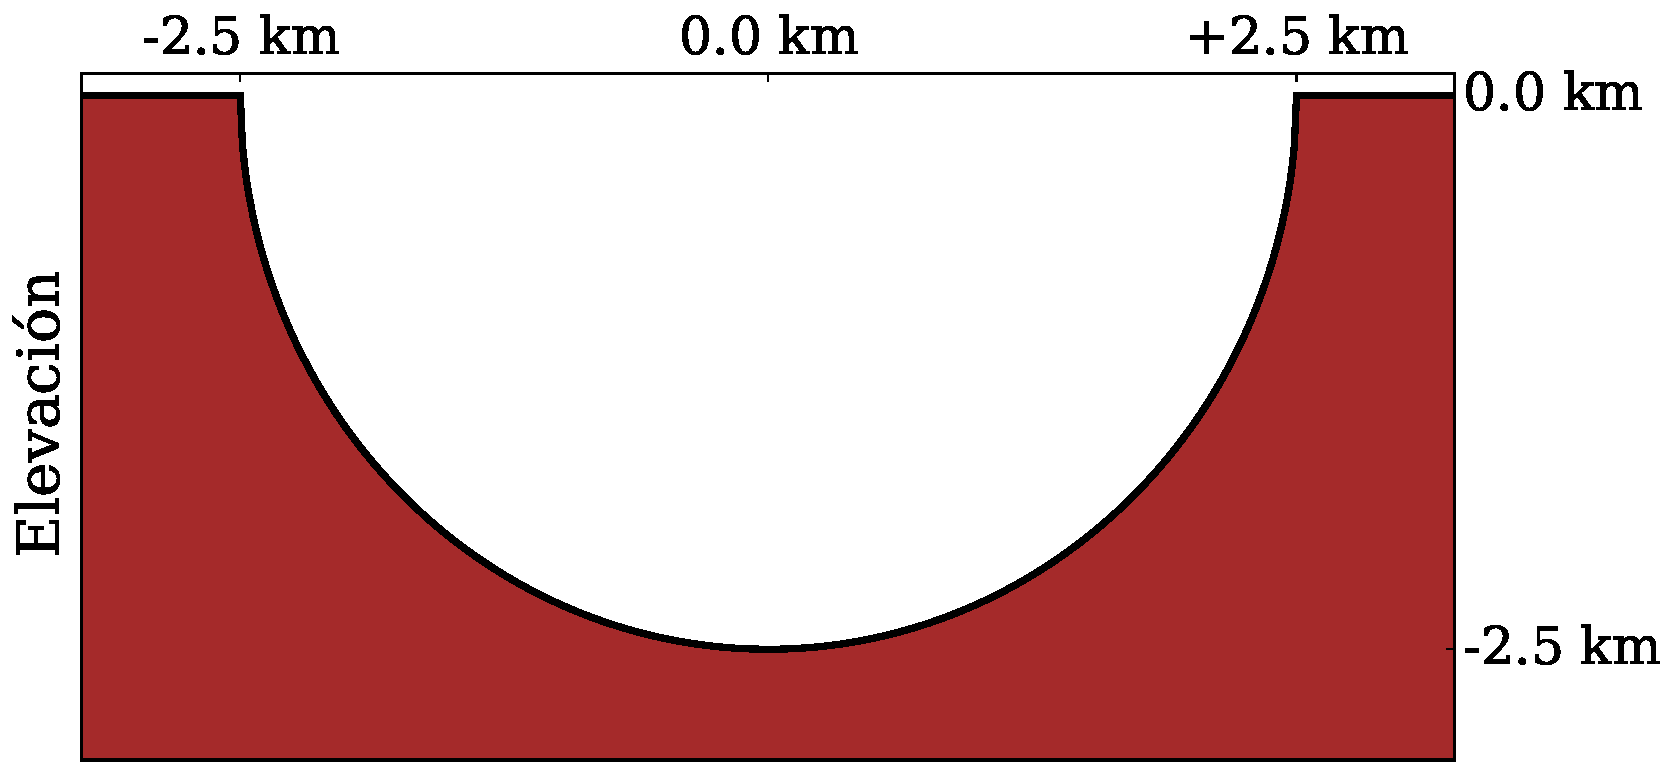
\includegraphics[width=8 cm]{img/ModelRegional.pdf}}
	\vspace{-.5 cm}
    \caption{Modelo 1.}
    \label{fig:model1}
    \vspace{-.5 cm}
\end{figure}
%
Inicialmente se analiza un modelo en el cual tanto la geometría regional como local tienen las mismas propiedades (modelo homogéneo). En el segundo modelo, la velocidad de propagación del material del dispersor local se definirá igual a la mitad del semiespacio.

En la \cref{fig:model1} se presentan los tres modelos analizados. La \cref{fig:model1}a corresponde al modelo completo, el cual contiene la topografía regional y local; la respuesta de este modelo será usada para verificar la eficiencia del método. La \cref{fig:model1}b corresponde al modelo de la topografía local, en este se asume que esta se encuentra sobre un semiespacio homogéneo en el cual la única irregularidad corresponde a la montaña, por lo tanto se desprecia la interacción entre la topografía local y la topografía regional. La \cref{fig:model1}c corresponde al modelo de la topografía regional en el cual se asume un medio homogéneo y se ha eliminado la topografía local quedando un semicírculo, en este modelo se desprecia la interacción entre la respuesta de la montaña y la geometría regional. 

En la \cref{fig:puntos} se muestra un acercamiento de la montaña dentro del modelo completo. En esta se muestran los puntos en los cuales se presenta la respuesta. Dentro del modelo regional, los puntos en los cuales se evalúa la respuesta corresponden a la proyección de los de la superficie de la montaña.

\begin{figure}[H]
	\centering
	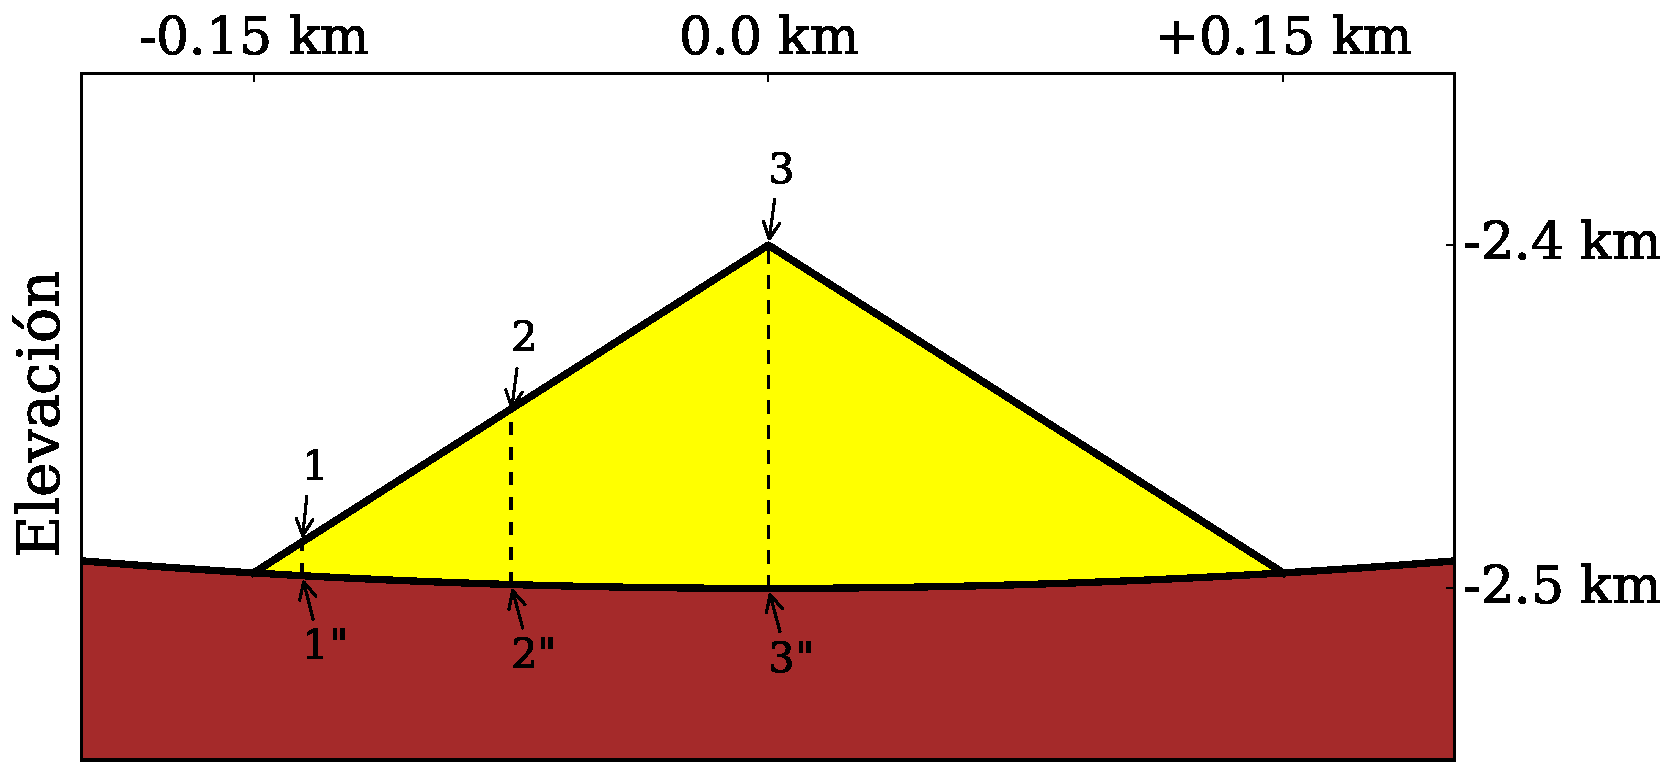
\includegraphics[width=12 cm]{img/ModelRegionalCompleteZoom.pdf}
	\vspace{-.5 cm}
	\caption{Puntos Evaluación Respuesta}
	\label{fig:puntos}
	\vspace{-1 cm}
\end{figure}
%

Los puntos sobre la superficie de la montaña se numeran como:
%
\begin{itemize}
%
	\item[1:] Esquina izquierda de la montaña.
	\vspace{-.5 cm}
	\item[2:] Mitad de la ladera.
	\vspace{-.5 cm}
	\item[3:] Vértice Superior
	\vspace{-.5 cm}
%
\end{itemize} 

Las proyecciones sobre el fondo del modelo regional se numeran como $1"$, $2"$ y $3"$.

Adicional a la respuesta de los tres modelos se presentará la respuesta del \textbf{\textit{``Modelo Local Modificado"}}, la cual se encuentra multiplicando la función de transferencia del modelo local por la del modelo regional.
%
%\begin{large}
	\begin{align}\label{eq:eqftmod}
		FT^{MLM} \left(\hat{i} \omega \right)= FT^{MR} \left(\hat{i} \omega \right) * FT^{ML} \left(\hat{i} \omega \right) 
		\vspace{-1 cm}
	\end{align}
%\end{large}
%
$FT^{MLM} \left(\hat{i} \omega \right)$ corresponde a la función de transferencia del modelo modificado, $FT^{MR} \left(\hat{i} \omega \right)$ es la función de transferencia del modelo regional y $FT^{ML} \left(\hat{i} \omega \right)$ la función de transferencia del modelo local.

Los elementos de los tres modelos se dimensionan según la \cref{eq:tamelem}:
%
%\begin{large}
	\begin{align}\label{eq:tamelem}
		\ell_{max} = \dfrac{\beta_{min}}{p  f_{max}}
 	\end{align}
%\end{large}
%
Donde $\ell_{max}$ corresponde al tamaño máximo de los elementos y $p$ corresponde al número de puntos por longitud de onda.
%
\subsection{Montaña Triangular Embebida en un Sector Semi-Circular, Modelo Homogéneo}
%
Para los tres modelos analizados se emplea la misma velocidad de onda de corte {$\beta = 1.0\ \text{km/s}$}, densidad $\rho = 1000\ \text{kg/m}^3$ y frecuencia máxima $f_{max} =  16\ \text{Hz}$. El sector semicircular tiene un radio $r=2.50\ \text{km}$, la montaña una base $b=0.30\ \text{km}$ y altura $h=0.10\ \text{km}$.

Para los tres modelos se emplean $24$ puntos por longitud de onda $\left( p = 24 \right)$.

En la \cref{fig:ftspatial} se muestran las funciones de transferencia sobre la superficie de los tres modelos de la \cref{fig:model1}, entre las coordenadas $-0.15\ \text{km}$ y $+0.15\ \text{km}$.\\
%
En la \cref{fig:ftspatial}a, la cual corresponde a una frecuencia igual a $0.20\ \text{Hz}$, no se observa variación espacial de la respuesta debido a que la longitud de onda es mucho mayor que la longitud sobre la cual se observa la respuesta. La respuesta del modelo local de la \cref{fig:model1}b tiende a la de un semiespacio, debido a que la longitud de onda es aproximadamente $17$ veces el ancho de la base de la montaña, $\lambda= 5.0\ \text{km}$, y la respuesta no se ve afectada por la presencia del dispersor; por esta misma razón, la respuesta del modelo regional y la del modelo completo son iguales.
%
\begin{figure}[H]
	\centering
	\subfloat []{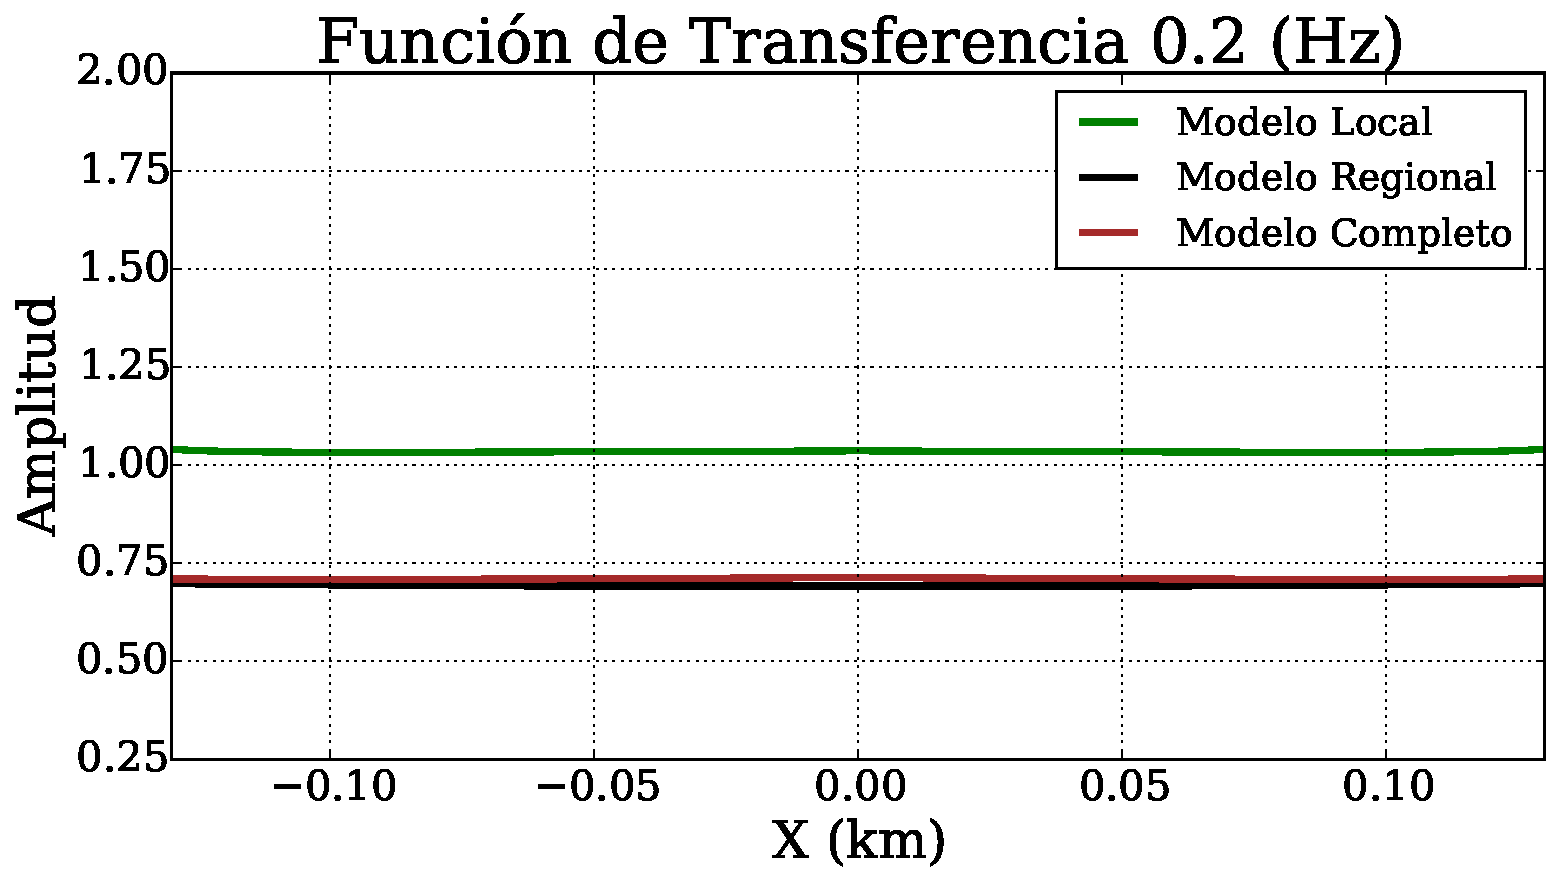
\includegraphics[width=8 cm]{img/TF_Homogeneo_2.pdf}}
	\subfloat []{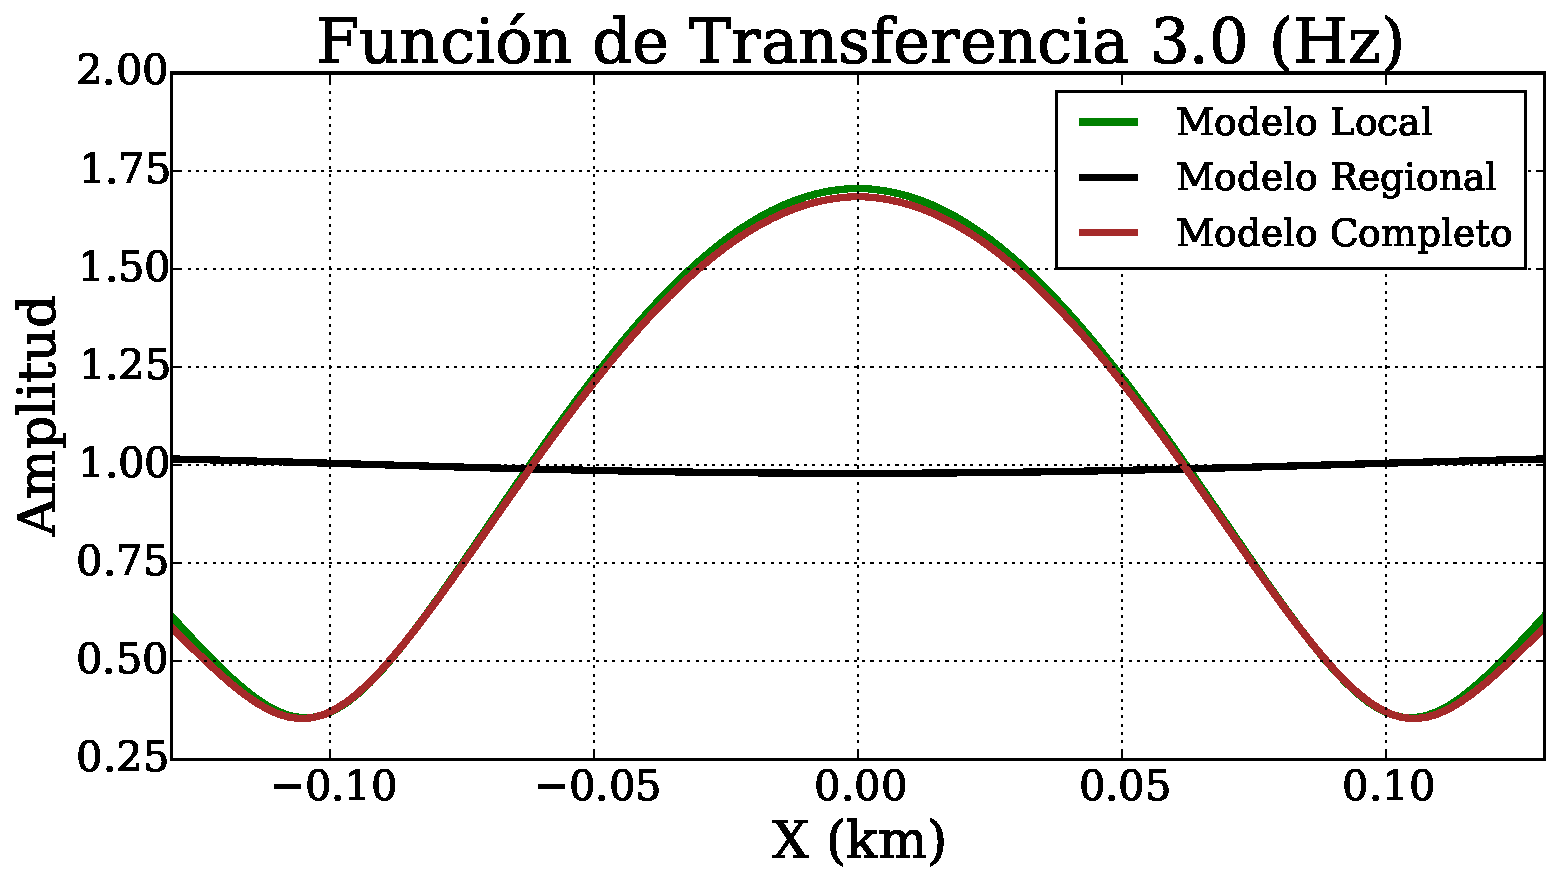
\includegraphics[width=8 cm]{img/TF_Homogeneo_30.pdf}}\\
	\vspace{-.5 cm}
	%
    \caption{Funciones de Transferencia Espaciales Modelos Homogéneos.}
    \label{fig:ftspatial}
    \vspace{-1 cm}
\end{figure}
%
En la \cref{fig:ftspatial}b, la cual corresonde a una frecuencia igual a $3.0\ \text{Hz}$, se observa una variación espacial para la respuesta de los modelos que contienen la geometría local debido a que en dicha frecuencia la longitud de onda es aproximadamente igual a la base de la montaña, $\lambda = 0.33\ \text{km}$. La respuesta del modelo regional tiende a la de un semiespacio debido a que la baja longitud de onda ve todo el dominio como un semiespacio.

En la \cref{fig:tfhom} se muestran la funciones de transferencia sobre las tres ubicaciones de la superficie de los modelos analizados, ver \cref{fig:puntos}. 

Como se mostró en el planteamiento del problema, la respuesta regional presenta una fuerte variación en la baja frecuencia, pero tiende a la respuesta de un semiespacio en la alta frecuencia. Esto refuerza la idea de que solo es necesario evaluar la respuesta en la baja frencuencia de la topografía regional, ya sea con modelo analíticos, semi-analíticos o computacionales.\\
%
La respuesta del modelo local se aproxima más a la respuesta de un semiespacio en la baja frecuencia, alejandose de esta a medida que la frecuencia aumenta. La respuesta en la baja frecuencia del modelo regional será la encargada de modificar la respuesta del modelo local, lograndose el objetivo de considerar el efecto regional en los estudios de efectos de sitio.\\
%
Coherente con los resultados anteriores, la respuesta del modelo completo presenta un comportamiento similar al del modelo regional en la baja frecuencia y al del modelo local en la alta frecuencia.\\
%
La respuesta del modelo local modificado se aproxima bastante bien a la respuesta del modelo completo, lo cual muestra que al menos para este modelo simplificado es bastante buena la aproximación dada por la \cref{eq:eqftmod}.

\begin{figure}[H]
	\centering
	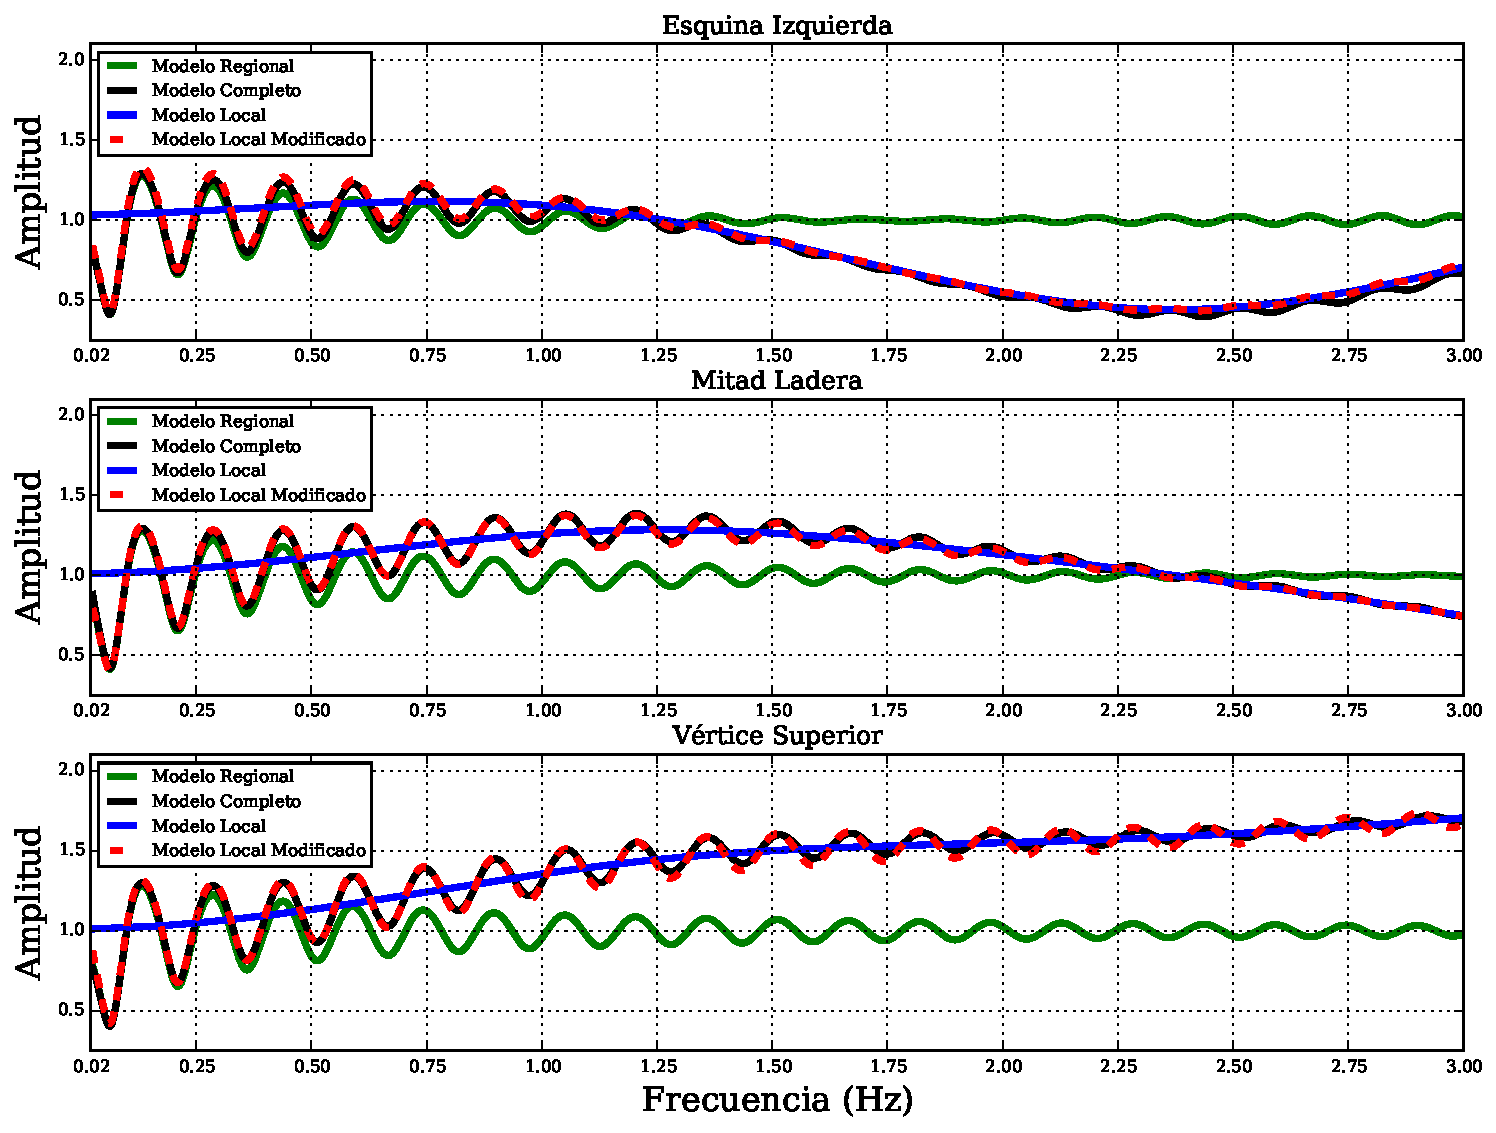
\includegraphics[width=15 cm]{img/TransFuncHom.pdf}
	\vspace{-.5 cm}
	\caption{Funciones de Transferencia Modelos Homogéneos}
	\label{fig:tfhom}
	\vspace{-1 cm}
\end{figure}
%
%
%
%
%
\subsection{Montaña Triangular Embebida en un Sector Semi-Circular, Modelo Inhomogéneo}
%
Para el semiespacio se define una velocidad de propagación de onda de corte $\beta_{HS} = 1.00\ \text{km/s}$, la del dispersor tipo montaña se define igual a la mitad de la del semi espacio $\beta_{Dispersor} = 0.50\ \text{km/s}$, se emplea la misma densidad $\rho = 1000\ \text{kg/m}^3$ para los materiales presentes en el dominio y se usa una frecuencia máxima $f_{max} =  16\ \text{Hz}$. Al igual que en el caso anterior, el sector semicircular tiene un radio $r=2.50\ \text{km}$, la montaña tiene una base $b=0.30\ \text{km}$ y altura $h=0.10\ \text{km}$.

Para los tres modelos se emplean $12$ puntos por longitud de onda $\left( p = 12 \right)$ para mantener la misma cantidad de elementos del caso anterior.

En la \cref{fig:ftspatialIn} se muestran las funciones de transferencia sobre la superficie de los tres modelos de la \cref{fig:model1}, entre las coordenadas $-0.15\ \text{km}$ y $+0.15\ \text{km}$.\\
%
En la \cref{fig:ftspatialIn}a al igual que en la \cref{fig:ftspatial}, no se observa variación espacial de la respuesta. La respuesta del modelo local de la \cref{fig:model1}b tiende a la de un semiespacio dado que la longitud de onda es aproximadamente $8$ veces el ancho de la base de la montaña la cual es bastante grande, $\lambda= 2.50\ \text{km}$, y la respuesta no ve el dispersor; por esta misma razón, la respuesta del modelo regional y la del modelo completo son casi iguales.
%
\begin{figure}[H]
	\centering
	\subfloat []{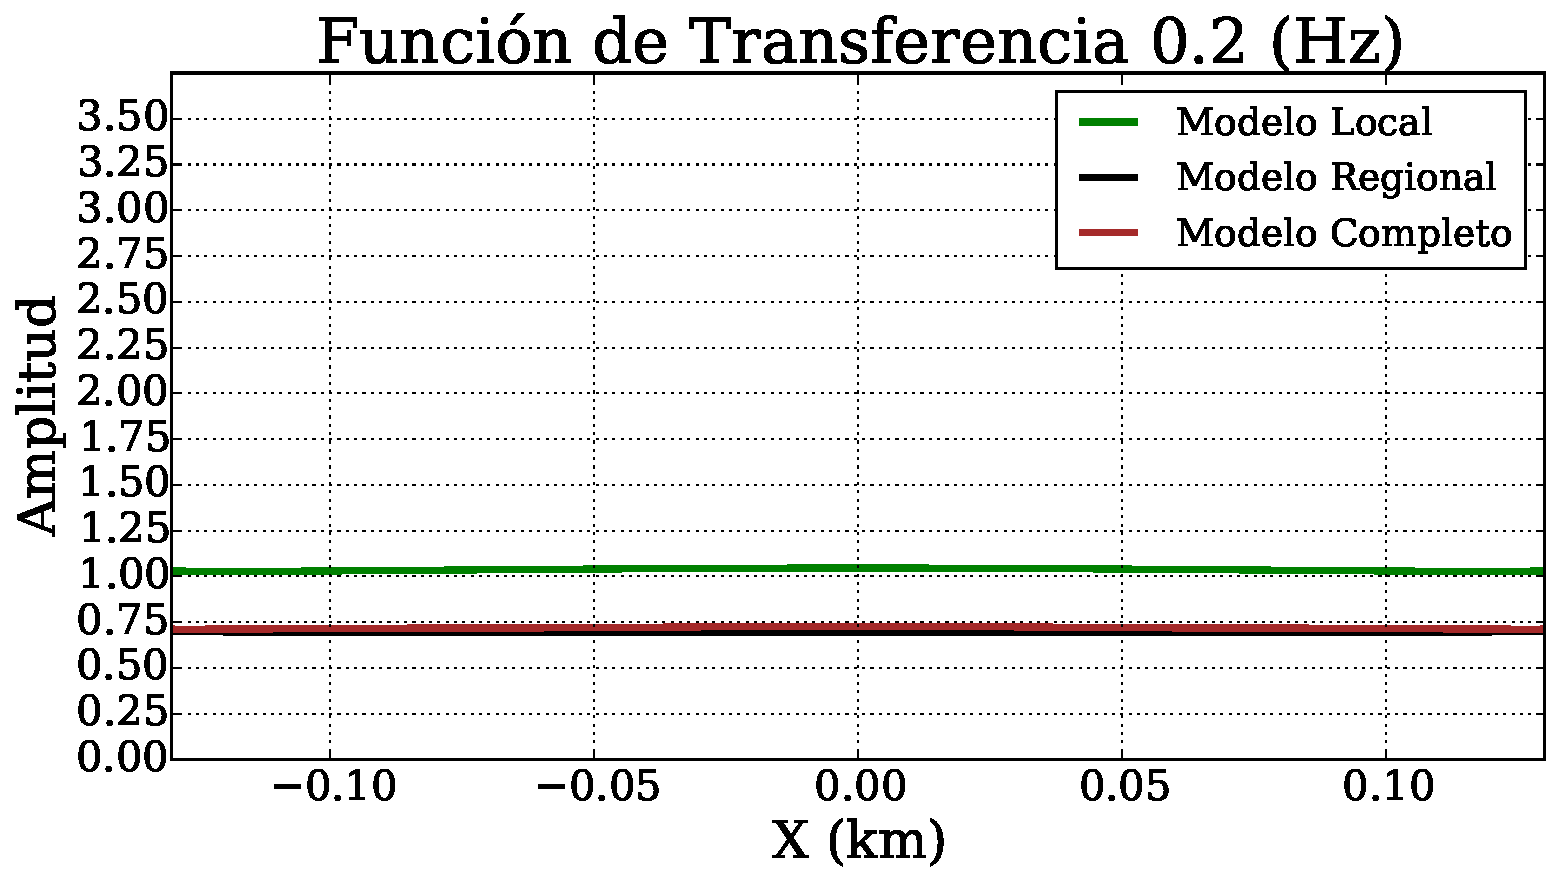
\includegraphics[width=8 cm]{img/TF_InHomogeneo_2.pdf}}
	\subfloat []{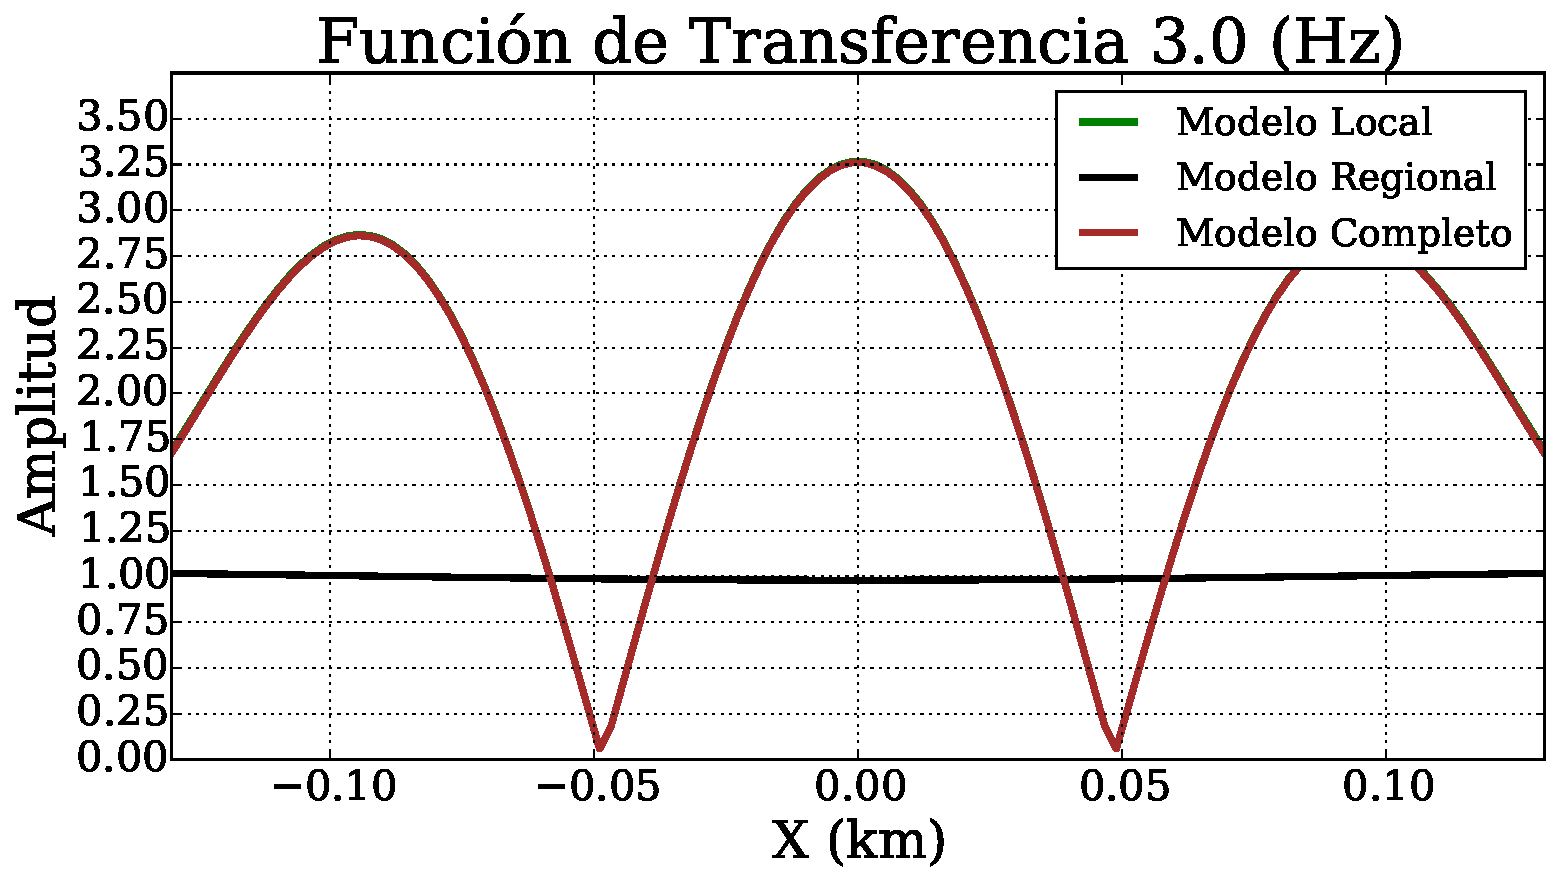
\includegraphics[width=8 cm]{img/TF_InHomogeneo_30.pdf}}\\
	\vspace{-.5 cm}
	%
    \caption{Funciones de Transferencia Espaciales Modelos Inhomogéneos.}
    \label{fig:ftspatialIn}
    \vspace{-1 cm}
\end{figure}
%
En la \cref{fig:ftspatialIn}b se observa una variación espacial mucho mayor a la de la \cref{fig:ftspatial}b debido a que en este modelo la longitud de onda es aproximadamente igual a la mitad de la base de la montaña, $\lambda = 0.167\ \text{km}$. Como en esta figura se muestra la amplitud de la función de transferencia, la distancia entre dos picos consecutivos corresponde a la mitad de la longitud de onda, por lo tanto a medida que aumenta la frecuencia se presenta una mayor variación espacial de la respuesta.

En la \cref{fig:tfinhom} se muestran la funciones de transferencia sobre las tres ubicaciones de la superficie de los modelos analizados, ver \cref{fig:puntos}. De esta figura se pueden sacar las mismas conclusiones del modelo anterior, lo cual indica que el método funciona bien aún en presencia de efecto acoplado suelo topografía.

\begin{figure}[H]
	\centering
	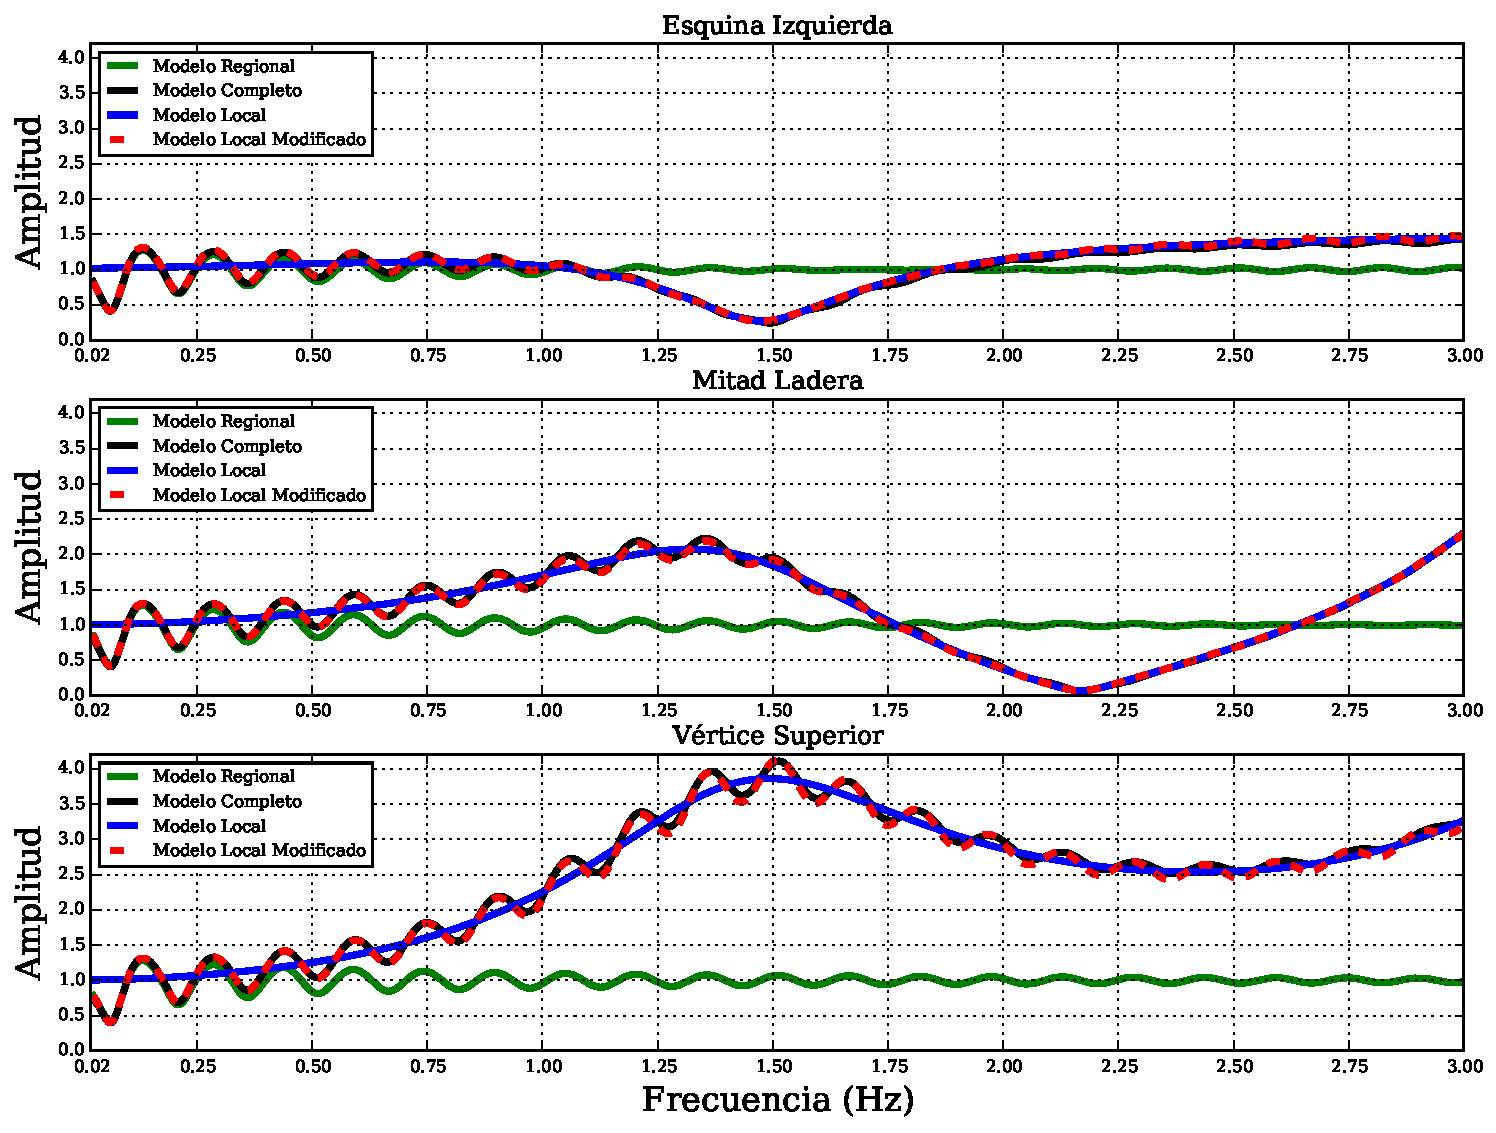
\includegraphics[width=15 cm]{img/TransFuncInHom.pdf}
	\vspace{-.5 cm}
	\caption{Funciones de Transferencia Modelos Inhomogéneos}
	\label{fig:tfinhom}
	\vspace{-1 cm}
\end{figure}
%
%
%
%
%
\newpage
%
\section{Trabajo Futuro}
%
Under construction
%
\bibliographystyle{gji}
\bibliography{refproposal}


\end{document}
